
\documentclass[notoc,nofonts,a4paper,oneside,nobib]{tufte-book}
%\documentclass[nofonts,a4paper,twoside]{book}

\usepackage{currfile,hyperxmp}

\usepackage{filemod}
   
\usepackage[
    type={CC},
    modifier={by-sa},
    version={4.0},
    imagewidth = 20mm,
    imageposition = left,
    imagedistance = -50mm,
]{doclicense}


\usepackage[refsegment=chapter,style=authoryear-comp,natbib=true]{biblatex}

\addbibresource{literature.bib}



\usepackage{amssymb,amsmath}
\usepackage{pgfplots}
    \usepackage{standalone}

\usepackage[T1]{fontenc}
\usepackage[utf8]{inputenc}


\usepackage{graphicx}
\setkeys{Gin}{width=\linewidth,totalheight=\textheight,keepaspectratio}


\usepackage{booktabs}
\usepackage{url}
\usepackage{hyperref}

\usepackage{units}

\usepackage{chemformula}

\usepackage{braket}
\setcounter{secnumdepth}{0}

% citations
%\usepackage{natbib}
%\bibliographystyle{plainnat}
%\setcitestyle{round} 

% pandoc syntax highlighting
%\usepackage{color}
%\usepackage{fancyvrb}



% longtable
\usepackage{longtable,booktabs}
\usepackage{multicol}
\usepackage[normalem]{ulem}

% morefloats
\usepackage{morefloats}




%% -- tint overrides
%% fonts, using roboto (condensed) as default
\usepackage[sfdefault,condensed]{roboto}
%% also nice: \usepackage[default]{lato}

%% colored links, setting 'borrowed' from RJournal.sty with 'Thanks, Achim!'
\RequirePackage{color}
\definecolor{link}{rgb}{0.1,0.1,0.8} %% blue with some grey
\hypersetup{
  colorlinks,%
  citecolor=link,%
  filecolor=link,%
  linkcolor=link,%
  urlcolor=link
}

%% macros
\makeatletter

%% -- tint does not use italics or allcaps in title
\renewcommand{\maketitle}{%     
  \newpage
  \global\@topnum\z@% prevent floats from being placed at the top of the page
  \begingroup
    \setlength{\parindent}{0pt}%
    \setlength{\parskip}{4pt}%
    \let\@@title\@empty
    \let\@@author\@empty
    \let\@@date\@empty
    \ifthenelse{\boolean{@tufte@sfsidenotes}}{%
      %\gdef\@@title{\sffamily\LARGE\allcaps{\@title}\par}%
      %\gdef\@@author{\sffamily\Large\allcaps{\@author}\par}%
      %\gdef\@@date{\sffamily\Large\allcaps{\@date}\par}%
      \gdef\@@title{\begingroup\fontseries{b}\selectfont\LARGE{\@title}\par}%
      \gdef\@@author{\begingroup\fontseries{l}\selectfont\Large{\@author}\par}%
      \gdef\@@date{\begingroup\fontseries{l}\selectfont\Large{\@date}\par}%
    }{%
      %\gdef\@@title{\LARGE\itshape\@title\par}%
      %\gdef\@@author{\Large\itshape\@author\par}%
      %\gdef\@@date{\Large\itshape\@date\par}%
      %\gdef\@@title{\begingroup\fontseries{b}\selectfont\LARGE\@title\par\endgroup}%
      %\gdef\@@author{\begingroup\fontseries{l}\selectfont\Large\@author\par\endgroup}%
      %\gdef\@@date{\begingroup\fontseries{l}\selectfont\Large\@date\par\endgroup}%
      \gdef\@@title{\begingroup\fontseries{b}\fontsize{28}{60}\selectfont\@title\par\endgroup}%
      \gdef\@@author{\begingroup\fontseries{l}\fontsize{16}{20}\selectfont\@author\par\endgroup}%
      \gdef\@@date{\begingroup\fontseries{l}\fontsize{16}{20}\selectfont\@date\par\endgroup}%
    }%
    %\phantom{XXX}%
    \vspace{12pc}%
    \@@title%
    \vspace{4pc}%
    \@@author
    \@@date
  \endgroup
  \thispagestyle{plain}% suppress the running head
  \tuftebreak% add some space before the text begins
  \@afterindentfalse\@afterheading% suppress indentation of the next paragraph
}

%% -- tint does not use italics or allcaps in section/subsection/paragraph
\titleformat{\chapter}%
  [display]% shape
  {\relax\ifthenelse{\NOT\boolean{@tufte@symmetric}}{\begin{fullwidth}}{}}% format applied to label+text
  %{\itshape\huge\thechapter}% label
  {\huge Chapter \thechapter}% label
  {0pt}% horizontal separation between label and title body
  %{\huge\rmfamily\itshape}% before the title body
  {\fontseries{b}\selectfont\huge}% before the title body
  [\ifthenelse{\NOT\boolean{@tufte@symmetric}}{\end{fullwidth}}{}]% after the title body

\titleformat{\section}%
  [hang]% shape
  %{\normalfont\Large\itshape}% format applied to label+text
  {\fontseries{b}\selectfont\Large}% format applied to label+text
  {\thesection}% label
  {1em}% horizontal separation between label and title body
  {}% before the title body
  []% after the title body

\titleformat{\subsection}%
  [hang]% shape
  %{\normalfont\large\itshape}% format applied to label+text
  {\fontseries{m}\selectfont\large}% format applied to label+text
  {\thesubsection}% label
  {1em}% horizontal separation between label and title body
  {}% before the title body
  []% after the title body

\titleformat{\paragraph}%
  [runin]% shape
  %{\normalfont\itshape}% format applied to label+text
  {\fontseries{l}\selectfont}% format applied to label+text
  {\theparagraph}% label
  {1em}% horizontal separation between label and title body
  {}% before the title body
  []% after the title body

%% -- tint does not use italics here either
% Formatting for main TOC (printed in front matter)
% {section} [left] {above} {before w/label} {before w/o label} {filler + page} [after]
\ifthenelse{\boolean{@tufte@toc}}{%
  \titlecontents{part}% FIXME
    [0em] % distance from left margin
    %{\vspace{1.5\baselineskip}\begin{fullwidth}\LARGE\rmfamily\itshape} % above (global formatting of entry)
    {\vspace{1.5\baselineskip}\begin{fullwidth}\fontseries{m}\selectfont\LARGE} % above (global formatting of entry)
    {\contentslabel{2em}} % before w/label (label = ``II'')
    {} % before w/o label
    {\rmfamily\upshape\qquad\thecontentspage} % filler + page (leaders and page num)
    [\end{fullwidth}] % after
  \titlecontents{chapter}%
    [0em] % distance from left margin
    %{\vspace{1.5\baselineskip}\begin{fullwidth}\LARGE\rmfamily\itshape} % above (global formatting of entry)
    {\vspace{1.5\baselineskip}\begin{fullwidth}\fontseries{m}\selectfont\LARGE} % above (global formatting of entry)
    {\hspace*{0em}\contentslabel{2em}} % before w/label (label = ``2'')
    {\hspace*{0em}} % before w/o label
    %{\rmfamily\upshape\qquad\thecontentspage} % filler + page (leaders and page num)
    {\upshape\qquad\thecontentspage} % filler + page (leaders and page num)
    [\end{fullwidth}] % after
  \titlecontents{section}% FIXME
    [0em] % distance from left margin
    %{\vspace{0\baselineskip}\begin{fullwidth}\Large\rmfamily\itshape} % above (global formatting of entry)
    {\vspace{0\baselineskip}\begin{fullwidth}\fontseries{m}\selectfont\Large} % above (global formatting of entry)
    {\hspace*{2em}\contentslabel{2em}} % before w/label (label = ``2.6'')
    {\hspace*{2em}} % before w/o label
    %{\rmfamily\upshape\qquad\thecontentspage} % filler + page (leaders and page num)
    {\upshape\qquad\thecontentspage} % filler + page (leaders and page num)
    [\end{fullwidth}] % after
  \titlecontents{subsection}% FIXME
    [0em] % distance from left margin
    %{\vspace{0\baselineskip}\begin{fullwidth}\large\rmfamily\itshape} % above (global formatting of entry)
    {\vspace{0\baselineskip}\begin{fullwidth}\fontseries{m}\selectfont\large} % above (global formatting of entry)
    {\hspace*{4em}\contentslabel{4em}} % before w/label (label = ``2.6.1'')
    {\hspace*{4em}} % before w/o label
    %{\rmfamily\upshape\qquad\thecontentspage} % filler + page (leaders and page num)
    {\upshape\qquad\thecontentspage} % filler + page (leaders and page num)
    [\end{fullwidth}] % after
  \titlecontents{paragraph}% FIXME
    [0em] % distance from left margin
    %{\vspace{0\baselineskip}\begin{fullwidth}\normalsize\rmfamily\itshape} % above (global formatting of entry)
    {\vspace{0\baselineskip}\begin{fullwidth}\fontseries{m}\selectfont\normalsize\rmfamily} % above (global formatting of entry)
    {\hspace*{6em}\contentslabel{2em}} % before w/label (label = ``2.6.0.0.1'')
    {\hspace*{6em}} % before w/o label
    %{\rmfamily\upshape\qquad\thecontentspage} % filler + page (leaders and page num)
    {\upshape\qquad\thecontentspage} % filler + page (leaders and page num)
    [\end{fullwidth}] % after
}{}

% tint: no smallcaps in header 
% The 'fancy' page style is the default style for all pages.
\fancyhf{} % clear header and footer fields
\ifthenelse{\boolean{@tufte@twoside}}
  %{\fancyhead[LE]{\thepage\quad\smallcaps{\newlinetospace{\plainauthor}}}%
  %  \fancyhead[RO]{\smallcaps{\newlinetospace{\plaintitle}}\quad\thepage}}
  %{\fancyhead[RE,RO]{\smallcaps{\newlinetospace{\plaintitle}}\quad\thepage}}
  {\fancyhead[LE]{\thepage\quad{\newlinetospace{\plaintitle}}}%
    \fancyhead[RO]{{\newlinetospace{\plaintitle}}\quad\thepage}}%
  {\fancyhead[RE,RO]{{\newlinetospace{\plaintitle}}\quad\thepage}}
  



\makeatother





%\makeatletter
\fancypagestyle{mystyle}{%
\fancyhf{}%
\fancyfoot[L]{\doclicenseThis}% 
}
%\makeatother

\usepackage{etoolbox}
\patchcmd{\chapter}{\thispagestyle{plain}}{\thispagestyle{mystyle}}{}{}



\hypersetup{
 linktocpage,
  colorlinks,
  citecolor=Maroon,
  filecolor=Maroon,
  linkcolor=RoyalBlue,
  urlcolor=RoyalBlue
}

\newcommand{\addtochapter}{%
\vspace*{-12mm}{
\setlength{\parindent}{0pt}
Markus Lippitz \newline \Filemodtoday{\currfilepath}
}
\vspace*{12mm}
}

\makeatletter
\let\stdchapter\chapter
\renewcommand*\chapter{%
  \@ifstar{\starchapter}{\@dblarg\nostarchapter}}
\newcommand*\starchapter[1]{\stdchapter*{#1}}
\def\nostarchapter[#1]#2{\stdchapter[{#1}]{#2} \addtochapter}
\makeatother


\begin{document}


\title{Experiments in Spectroscopy}

\author{Markus Lippitz}
\date{\today}


\maketitle



\tableofcontents

\part{Fundamentals}

%\renewcommand{\lastmod}{April 29, 2020}

\chapter{Absorption}




\section{Tasks}

\begin{itemize}
\item Get acquainted with the different measures for absorption and how they relate. Starting from the experimental values in the following papers, calculate all other measures.

\begin{tabular}{ll}
InGaAs quantum dots & \cite{Borri:2002p139}, last page  \\
CdSe nanocrystals & \cite{Jasieniak:2009er}, Fig. 2 and 3 \\
xanthene dye & \cite{Kastrup:2004p1737}, Fig. 4d   \\
MEH-PPV conjugated polymer  & \cite{Hou:2017jm}, Fig. 3 \\
\end{tabular}


\item Get a feeling for typical absolute values and compare them to relevant  other quantities, such as geometrical size, bond lengths, transition rates etc. Sometimes it makes sense to factor out some constants and compare only then.
\item Why are there so many different measures for absorption? Find use cases where it makes especially sense to use one measure and not the others.

\end{itemize}







%\section{Experiment}
\section{Experimental technique}

An UV/VIS spectrometer measures the  power $P$ transmitted through a cuvette of optical path length $L$ and compares it to the power $P_0$ in a reference path. In most cases, also here, the reference path holds a cuvette containing  the plain solvent. The transmission $T = P / P_0$ is converted into the absorbance $A = - \log_{10} T = - \log_{10} ( P / P_0)$. The data set gives absorbance as function of wavelength.

\begin{marginfigure}
\inputtikz{\currfiledir uvvis}
\caption{Sketch of a UV/VIS spectrometer}
\end{marginfigure}



Grating spectrometers use an entrance slit to define the spectral resolution $d \lambda$, which is independent of the actual wavelength $\lambda$, as can be seen when inspecting the   angular dispersion relation of a grating. Due to the reciprocal relation between wavelength and frequency or energy, the spectral resolution in units of energy $d \nu$ is not constant anymore.




\section{Lambert-Beer law and the absorption coefficient}

The transmitted power drops exponentially with  concentration $C$ and  path length $L$
\begin{equation}
 P = P_0 \, 10^{- \epsilon\, C \, L}
\end{equation}
where $\epsilon$ is the (decadic) molar absorption\sidenote{The difference between abortion and extinction will be discussed elsewhere.} coefficient. We stick here to a base of $10$, 
so that the absorbance or optical density equals 
\begin{equation}
 A = \epsilon\, C \, L \quad.
\end{equation}
However, similar definitions with a base of $e$ are used sometimes. Our choice leads to the appearance of factors of $\ln(10)$ every now and then. The concentration is typically given as molarity (1 M = 1 mol/l), and lengths for practical reasons in centimeter
so that the molar absorption coefficient has the unit 1/(M  cm). As we are concerned with spectroscopy the molar absorption coefficient $\epsilon$ depends of course on the wavelength or frequency of light.

\section{Absorption cross section}


The interaction cross section $\sigma$ of a process is an imagined area around the particle, which, when hit by a photon, triggers the considered process. When a photon hits on the absorption cross section $\sigma_{\text{abs}}$ of a molecule it will be absorbed. If it does not hit it will pass unperturbed. All details of the physics are summarized in the area, which makes it easy to relate the absorption cross section with the absorbance. 
\begin{marginfigure}
\inputtikz{\currfiledir crosssection}
\caption{Sketch  disks hit by rays}
\end{marginfigure}


We consider randomly arranged molecules of molar concentration $C$ in a thin slab of thickness $dx$. The probability that a photon is absorbed in this slab is
\begin{equation}
 1 - T =1 -  10^{- \epsilon\, C \, dx} \approx \ln (10) \; \epsilon\, C \, dx \quad .
\end{equation}
In comparison, when each molecule has an absorption cross section $\sigma_{\text{abs}}$, we get an absorption probability 
\begin{equation}
 1 - T = \sigma_{\text{abs}} \, C \, N_A \, dx
\end{equation}
where $N_A = 6.022 \cdot 10^{23}$~{1/mol} is the Avogadro number.  We also made the Born approximation, i.e., that multiple interactions can be neglected, or the absorption cross sections do not overlap, which is equivalent to the approximation made above to remove the exponential function.  We thus find
\begin{equation}
 \sigma_{\text{abs}}(\omega) =  \frac{\ln(10)}{ N_A } \, \epsilon(\omega)
\end{equation}
which has the unit of an area. As the  molar absorption coefficient $\epsilon$  also the absorption cross section $\sigma_{\text{abs}}$ depends on the wavelength of light. If no wavelength is given, the value at the peak of the spectrum is meant.


\section{Lorentz oscillator and oscillator strength}


\begin{marginfigure}
\inputtikz{\currfiledir mass_spring}
\caption{A Lorentz oscillator}
\end{marginfigure}


The Lorentz oscillator is a simple classical model to describe the interaction of light and matter. A mass $m$ of charge $+e$ is connected to a spring. The oscillator has an angular eigen-frequency $\omega_0$ and a damping $\gamma$. It is driven by an external electrical field $E(t) = E_0 \exp(i \omega t)$. The differential equation for the position $x$ reads
\begin{equation}
  \ddot{x} + 2  \gamma  \dot{x} + \omega_0^2 x =  \frac{e}{m} E_0 e^{i \omega t}
\end{equation}
This results in a steady-state solution of \sidenote{check: should be $-i\gamma$ for Lorentz osci}
\begin{equation}
  x(t) = \frac{e}{m}  \frac{1}{\omega_0^2 - \omega^2 + 2  i \gamma \omega } \, E_0 e^{i \omega t} 
\end{equation}
In the case of small damping ($\gamma \ll \omega_0$) this simplifies near the resonance ($\omega \approx \omega_0$) to
\begin{equation}
  x(t) \approx \frac{e}{2 m \omega_0}  \frac{1}{\omega_0 - \omega + i \gamma } \, E_0 e^{i \omega t} 
\end{equation}
The time-averaged power  that the damped oscillator takes out of the driving force $F(t) = e E(t)$ can be calculated in this approximation as
%
\begin{eqnarray}
 P_{\text{abs}} &= &  - \frac{1}{T} \int_0^T F \, \frac{ds}{dt} \, dt =  
  - \frac{1}{T}  \int_0^T Re \left\{  e E(t) \right\}  \, Re \left\{ \dot{x}(t) \right\} \, dt \\
  & = & - Re \left\{i \omega  \frac{e^2  E_0^2 }{2 m \omega_0}  \frac{1}{\omega_0 - \omega +  i \gamma } \right\}  \,   \frac{1}{T}  \int_0^T \left( \cos \omega t \right)^2 dt \\
 % 
%
% P_{\text{abs}} &= & \left< Re \left\{ e E(t) \, \dot{x}(t) \right\} \right> = 
 %
 % & = & Re \left\{ \frac{i \omega}{2} \frac{e^2  E_0^2 }{2 m \omega_0}  \frac{1}{\omega_0 - \omega +  i \gamma } \right\}  \\
%& \approx & Im \left( \frac{e^2  E_0^2 }{4 m }  \frac{1}{\omega_0 - \omega + i \gamma }  \right)
& = & \frac{e^2 E_0^2  }{4 m }  \frac{\gamma }{(\omega_0 - \omega)^2 +  \gamma ^2}  \\
&  = &  \frac{e^2  }{2 \epsilon_0 \, m \,c }  \frac{\gamma }{(\omega_0 - \omega)^2 +  \gamma ^2}  \, |S|  \quad .
\end{eqnarray}
%
The time average has produced a factor of $1/2$ and in the last step we have used the definition of the amplitude of the Poynting vector $|S| = \frac{1}{2} \epsilon_0 c |E_0|^2$. 
We thus find an absorption cross section $\sigma_{\text{abs,Lorenz}}$ of the classical Lorentz oscillator
\begin{equation}
 \sigma_{\text{abs, Lorentz}}(\omega) = \frac{ P_{\text{abs}} }{|S| } = \frac{e^2  }{2 \epsilon_0 \,  m \, c}  \frac{\gamma }{(\omega_0 - \omega)^2 +  \gamma ^2} 
\end{equation}

While many optical transitions show a Lorentzian line shape as predicted by the Lorentz oscillator, the peak height of the absorption line deviates. This deviation is cast into an oscillator strength $f$ so that 
\begin{equation}
 \sigma_{\text{abs}}(\omega) =   \frac{e^2  }{2 \epsilon_0 \,  m \, c}  \frac{\gamma  }{(\omega_0 - \omega)^2 +  \gamma ^2}  \, f
\end{equation}

For single electron transitions starting from the same quantum mechanical level, the Thomas–Reiche–Kuhn sum rule states that the sum over all oscillator strength $f$ equals to one. For this reason, one can interpret the oscillator strength  $f$  to some extent  as the number of electrons involved in  the transition, but one has to be careful, as pointed out by Z. Hens \footcite{Hens:2008kr}.

The spectral integral of the absorption cross section is independent of its width $\gamma$ as
\begin{equation}
 \int \sigma_{\text{abs}}(\omega)  \, d \omega =
   \frac{\pi \, e^2  }{2 \epsilon_0 \,  m \, c} \, f
\end{equation}


\section{Transition dipole moment}

\begin{marginfigure}
\inputtikz{\currfiledir tls_absorption}
\caption{A light beam induces a transition from $\ket{i}$ to the  $\ket{f}$.}
\end{marginfigure}

Fermi's Golden Rule gives the transition rate from the initial state $\ket{i}$ to the final state $\ket{f}$ caused by the time-dependent perturbation $H'$ to the stationary Hamilton operator $H_0$ as
\begin{equation}
 \Gamma_{i \rightarrow f} = \frac{2 \pi}{\hbar} \, \left| \bra{f} H' \ket{i} \right|^2 \, \rho(E) \quad ,
\end{equation}
where  $\rho(E) = d n / d E = \rho(\omega) / \hbar$ is the density of final states. The idea is that the initial state  $\ket{i}$ is well known, but the outcome of the interaction $\ket{f}$ might have free parameters, for example the direction of the emitted electron or the mode of the absorbed photon. The density of states   $\rho(E)$ thus can describe either electronic or photonic states, or both.




In general, the interaction of a charged particle with an electromagnetic vector potential $\mathbf{A}$ is described by the perturbation
\begin{equation}
 H' = - \frac{i \hbar e}{m} \, \mathbf{A \cdot \nabla}  \quad .
\end{equation}
As the spatial extent of our wavefunctions is small compared to the wavelength of light, we employ the dipole approximation and assume $\exp( i \mathbf{k \cdot r}) \approx 1$ in the plane-wave description of the vector potential. In this way, the  perturbation operator $H'$ simplifies to\sidenote{see \textcite{bransden_joachain} for details}
\begin{equation}
 H' =  e \, \mathbf{E} (t)  \mathbf{\cdot \, r} =  e \,E_0 \,  \mathbf{\hat{x} \cdot \, r} \, \cos(\omega t) \quad ,
\end{equation}
where $\mathbf{\hat{x}} $ is a unit vector defining the polarization direction of the light field. We simplify further by using the rotating-wave approximation and keeping only co-rotating parts\sidenote{More on this in the chapter on Rabi oscillations and the Bloch sphere.} 
\begin{equation}
 \cos(\omega t)
 = \frac{1}{2} \left( e^{i \omega t}+  e^{-i \omega t} \right)
 \approx  \frac{1}{2}  e^{i \omega t} 
\end{equation}
so that 
\begin{equation}
H' =  \frac{ e \,E_0}{2}  \,  \mathbf{\hat{x} \cdot \, r} \,  e^{i \omega t}  \quad .
\end{equation}
%
 We introduce the transition dipole matrix element $\mu_{if}$ as
\begin{equation}
\mathbf{\mu}_{if} = -e \, \bra{f}    \mathbf{r} \ket{i}  \quad .
\end{equation}
It has the units of an electric dipole moment, i.e., charge times distance, and is the central element of an optical transition in quantum mechanics. For practical reasons, one uses the unit of 1 Debye = 1 electron displaced by 0.208 \AA.
With this the matrix element  becomes
\begin{equation}
\left| \bra{f} H' \ket{i} \right|^2 =  \frac{1}{4} E_0^2  \, |\mathbf{\hat{x}} \cdot \mathbf{\mu}_{if} |^2 \quad .
\end{equation}
Plugging everything into Fermi's Golden Rule, we get
\begin{equation}
 \Gamma_{i \rightarrow f} = \frac{\pi}{2 \hbar^2} \,  E_0^2  \, |\mathbf{\hat{x}} \cdot \mathbf{\mu}_{if} |^2 \, \rho(\omega) \quad .
\end{equation}
Now we have to take into account that we use a incoherent multimode light source.\sidenote{The effect of a coherent single mode source will be investigated in the context of Rabi oscillations.} The electric field $E$ is here an incoherent superposition of  modes with the  spectral energy density $u(\omega)$.\sidenote{see \textcite{CT} and \textcite{Fox}   for details}
The total power is thus
\begin{equation}
 \frac{1}{2} \epsilon_0  \, E_0^2  = \int  u(\omega)  \, d\omega \quad .
\end{equation}
The  transition rate is thus 
\begin{equation}
 \Gamma_{i \rightarrow f} =   \frac{\pi  }{\hbar^2 \epsilon_0}  \, |\mathbf{\hat{x}} \cdot \mathbf{\mu}_{if} |^2 \,
\int u(\omega)  
  \rho(\omega)  d \omega \quad .
\end{equation}
As the atomic transition is narrow compared with the light spectrum, the density of states $\rho(\omega)$ selects the transition frequency $\omega_{if}$ 
\begin{equation}
 \Gamma_{i \rightarrow f} =   \frac{\pi  }{\hbar^2 \epsilon_0}  \, |\mathbf{\hat{x}} \cdot \mathbf{\mu}_{if} |^2 \,
 u(\omega_{if})   \quad .
\end{equation}
As each absorption event takes out a photon of energy $\hbar \omega_{if}$, and the energy density moves with the speed of light $c$ we get an integrated absorption cross section $\sigma_{\parallel}$ 
\begin{equation}
 \int \sigma_{\parallel}(\omega) \, d \omega = \frac{ \hbar \omega_{if} \, \bar{\Gamma}_{i \rightarrow f} }{c \, u(\omega_{if})}  = 
  \frac{\pi \omega_{if}}{ \hbar c \, \epsilon_0} \,
 |\mathbf{\mu}_{if} |^2  \quad . \label{eq:abs_sigma_mu}
\end{equation}
The index ${\parallel} $ is necessary, as we dropped the dot product between the direction of the transition dipole moment $\mathbf{\mu}_{if}$ and the polarization direction $\mathbf{\hat{x}}$, assuming optimal parallel orientation. In case of random orientation, i.e., averaging over all possible orientation directions, one finds  a reduction by one third, i.e. $\sigma = 1/3 \sigma_{\parallel} $

We can recover the spectral resolved absorption cross section $\sigma_{\parallel}(\omega)$ by assuming a line-shape function $L(\omega - \omega_0)$ so that 
\begin{equation}
 \sigma_{\parallel}(\omega) =  \frac{\pi \omega_{if}}{ \hbar c \, \epsilon_0} \,
 |\mathbf{\mu}_{if} |^2 \, L(\omega - \omega_{if})
\end{equation}
where the integral over $L$ equals one. Assuming a Lorentzian line shape, the peak value of $L$ equals $1/(\pi \gamma)$ so that
\begin{equation}
 \sigma_{\parallel}(\omega_{if}) =  \frac{\omega_{if}}{ \hbar c \, \epsilon_0 \, \gamma} \,
 |\mathbf{\mu}_{if} |^2  \quad .
\end{equation}
In the chapter on fluorescence we will discuss the relation between the transition dipole moment $|\mathbf{\mu}_{if} |^2 $ and the Einstein $A$ and $B$ coefficients. When spontaneous emission is the only factor to influence the width of the optical transition (as for an atom in vacuum), we find
\begin{equation}
 \gamma = \frac{1}{2} A_{21} = \frac{\omega^3}{6 \pi \hbar c^3 \epsilon_0} |\mathbf{\mu}_{if} |^2  
\end{equation}
so that in this case the absorption cross section reduces to 
\begin{equation}
 \sigma_{\parallel}(\omega_{if}) =  \frac{3}{2 \pi} \, \lambda^2 \quad .
\end{equation}
The absorption cross section of an atom, molecule, nanocrystal is thus limited. However, as only in exceptional cases the line width is Fourier-limited, i.e. limited by the radiative decay, in most cases the absorption cross section is much smaller. The reduction is given by the ratio of the Fourier-limited line width to the observed width of the transition. 


When relating to the  (decadic) molar absorption coefficient $\epsilon(\omega)$ we have to realize that in the more 'atomic' contexts of transition dipole moments and Einstein coefficients, we integrated over the spectral width of the absorption line. We  assumed that the incoming light beam is spectrally much broader than the optical transition. This is not the case for molecular spectra at room temperature. We thus have to integrate also the absorption spectrum over $\omega$ and take into account that $\omega_{if}$ varies, so that
\begin{equation}
 \int_{\text{transition}} \frac{\epsilon(\omega)}{\omega} \, d \omega \, = \, 
  \frac{\pi \, N_A}{ 3 \, \ln(10) \, \hbar c \, \epsilon_0} \,
 |\mathbf{\mu}_{if} |^2
 \, = \, 
  \frac{\hbar\, N_A}{ \ln(10) \, c } \,
B_{12}  \quad .
\end{equation}




\section{Appendix: Thomas-Reiche-Kuhn sum rule}

Taken from Wikipedia. 
%
\begin{align}
& \sum_n (E_n-E_m)\left|\left\langle n | \hat x | m \right\rangle\right|^2 \\
&= \sum_n (E_n-E_m) \left\langle m\right |\hat x\left | n\right\rangle\left\langle n \right| \hat{x}\left | m\right\rangle\\
%
&=\frac{1}{2}\sum_n\left(\left\langle m\right | \hat{x}\hat{H}-\hat{H}\hat{x}\left |n\right\rangle\left\langle n \right | \hat{x}\left | m\right\rangle + \left\langle m \right | \hat{x}\left | n\right\rangle\left\langle n\right | \hat{H}\hat{x}-\hat{x}\hat{H}\left |m\right\rangle \right)\\
%
&=\frac{1}{2}\sum_n \left(\left\langle m\right | \hat{x}\left |n \right\rangle\left\langle n\right | [\hat{H},\hat{x}]\left|m\right\rangle-\left\langle m \right | [\hat{H},\hat{x}]\left | n \right\rangle\left\langle n\right|\hat{x}\left| m \right\rangle \right)\\
%
&=\frac{1}{2}\left( \left\langle m\right | \hat{x}[\hat{H},\hat{x}]\left | m \right\rangle -\left\langle m\right | [\hat{H},\hat{x}]\hat{x}\left |m\right\rangle \right)\\
&=\frac{1}{2} \left( \left\langle m \right | [\hat{x},[\hat{H},\hat{x}]] \left | m \right\rangle \right)\\
%
&= -\frac{i\hbar}{2m_0}\left\langle m\right| [\hat{x},\hat{p}]\left| m \right\rangle\\
%
&= \frac{\hbar^2}{2m_0}
\end{align}
%
using
\begin{equation}
[\hat{H},\hat{x}]=-\frac{i\hbar}{m_0}\hat{p} \quad \text{and} \quad  [\hat{x},\hat{p}]=i\hbar
\end{equation}
The dipole operator $\hat{\mu}$ is proportional to the position operator $\hat{x}$. The sum over all $|\mathbf{\mu}_{if}|^2$ starting from the same state $i$ is thus constant.

\section{Appendix: Units }

mass $M$, time $T$, length $L$, current $i$, particle number $mol$

\begin{tabular}{rl}
   $\epsilon_0$  & $i^2 T^4 / M L^3$ \\
    field $E_0$ & $M L / i T^3$ \\
    energy & $M L^2 / T^2$ \\
    $\mu_{if}$ & $ L i T$ \\
    $\omega$ & $1/T$ \\
    $u(\omega)$ & $M / T L$ \\
    $\hbar$ & $ M L^2 / T$ \\
    $\rho(\omega) $ & $T$ \\
    $\Gamma_{if}$ & $ 1/T$ \\
    $B_{12}$ & $ L / M$ \\
  $\epsilon(\omega)$ & $L^2 / mol$
\end{tabular}

\printbibliography[segment=\therefsegment,heading=subbibliography]

%\renewcommand{\lastmod}{May 1, 2020}


\chapter{Fluorescence}


\section{Tasks}

\begin{itemize}
\item On the server, you find experimental data of the TDI dye. Compare the fluorescence emission rate obtained from the emission spectrum with the fluorescence lifetime from time-correlated single photon counting. Discuss differences.

\item Find absolute values for other transition rates in atoms, molecules and solid state and compare to fluorescence rates.

\end{itemize}

\begin{marginfigure}
   \includestandalone[width=50mm]{\currfiledir fig_tdi}
  \caption{Absorption and emission spectrum of a dye molecule (TDI).}
\end{marginfigure}



\section{Experimental techniques}



\subsection{Measuring the spectrum of light}

It is helpful to consider how the spectrum of light is really measured. A light beam is dispersed, typically on a grating. As function of the dispersion angle one measures light intensity by converting photons into electrons, either in a CCD camera or a photodiode. The signal amplitude is thus proportional to the  photon rate, not the power, or the energy per photon.

The resolution of a grating spectrometer is determined by the width of the CCD pixels, the size of the diode or of the entrance slit, by the size of a monochromatic focus, or a combination of all. But in all cases, it is constant over the spectrum when measured in wavelength. The natural unit of a grating spectrometer is wavelength, not frequency. The reciprocal relation between wavelength and frequency leads to 
\begin{equation}
 \Delta \nu = \nu_2 - \nu_1 = \frac{c}{\lambda_2} - \frac{c}{\lambda_1}  = c \frac{\lambda_1 - \lambda_2}{\lambda_1 \lambda_2} \approx \frac{c}{\lambda^2} \, \Delta \lambda
\end{equation}
In the frequency domain, the spectral resolution is thus not constant, but proportional to $\nu^2$. As consequence, converting a data set from wavelength domain to frequency domain does not only entail converting the $x$-values, but also the $y$-values. The integral or total number of photons has to stay the same.
\begin{equation}
 \left( \lambda \, ; \, F(\lambda) \right) \, \rightarrow  \left( \nu = \frac{c}{ \lambda} \, ; \,  F(\nu) = \frac{\lambda^2}{ c } \, F(\lambda) \right) 
\end{equation}
This problem only occurs for spectra of light. Absorption spectra are the ratio of two spectra of light, of the signal and reference beam. In this case, the prefactors cancel out and only the $x$-values need to be converted. The spectrally integrated absorption does not have any meaning, in contrast to the spectrally integrated photon flux.



\subsection{Time correlated single photon counting}

\begin{marginfigure}
   \inputtikz{\currfiledir tcspc}
  \caption{Sketch of a TCSPC setup}
\end{marginfigure}

This technique measures the arrival time of single photons relative to the laser pulse that excites the sample. It requires that each laser pulse leads to on average much less than one detected photon. This can be achieved using weak laser pulses or diluted samples. A high repetition rate (MHz) reduces the overall acquisition time. The probability to detect a photon at a time lag $\tau$ after the laser pulse is directly connected to the probability, that the emitting system is still in the excited state. This statement does not require that each emitted photon is detected or that the excited state is depopulated only by fluorescence emission.





\section{Einstein coefficients}

\begin{marginfigure}
\inputtikz{\currfiledir einstein-coeff}
  \caption{Einstein coefficients}
\end{marginfigure}


The Einstein coefficients for emission $A_{21}$, absorption $B_{12}$ and stimulated emission $B_{21}$ relate the populations $N_1$ and $N_2$ of a lower and upper state to the spectral energy density $u(\omega)$ of the optical field (units of energy per volume and angular frequency interval). They define transition rates in units of Hz
\begin{eqnarray}
 k_{\text{spontaneous emission}} &=& A_{21} \\
  k_{\text{absorption}}  & = & B_{12} \,   u(\omega) \\
  k_{\text{stimulated emission }} & =&  B_{21} \,  u(\omega)  \quad .
\end{eqnarray}
%
In steady state we get
\begin{equation}
 \frac{d N_1}{dt} =  A_{21} N_2 \, - \, B_{12} \, N_1 \, u(\omega) \, + \, B_{21}\, N_2 \,u(\omega)  = 0 \quad .
\end{equation}
At the same time, the ratio of the populations is given by Boltzmann's law as
\begin{equation}
 \frac{N_2}{N_1} = \frac{g_2}{g_1} \, \exp \left( - \frac{\hbar \omega}{kT} \right)
\end{equation}
where the $g_i$ are the degeneracy of the respective state. The spectral energy density is given by the black-body spectrum, as we are in thermal equilibrium
\begin{equation}
 u(\omega) = \frac{\omega^2}{\pi^2 c^3} \, \hbar \omega \, \frac{1}{\exp \left( \hbar \omega / kT \right) - 1} \quad .
\end{equation}
Altogether this leads to 
\begin{eqnarray}
 g_1 \, B_{12} &=& g_2 \, B_{21} \\
 A_{21} &=&  \frac{\hbar \, \omega^3}{\pi^2 c^3} \, B_{21}  \label{eq:fl_Einstein_A_B}
\end{eqnarray}
Different prefactors can be found in literature for these equations, depending on the exact definition of $u$.
 \footcite{Hilborn:2002wj} 
 As each absorption event takes out the energy $\hbar \omega$ and the energy density $u(\omega)$ moves with the velocity of light $c$, we get for the absorption cross section
\begin{equation}
\int \sigma(\omega) \, d \omega = \frac{\hbar \omega_{12} \, B_{12} \, u(\omega_{12})  }{c \, u(\omega_{12}) }  =
   \frac{\hbar \omega_{12}  }{c  }    \, B_{12}
\end{equation}
assuming that almost all atoms are in the ground state ($N_2 \ll N_1$). Using \ref{eq:abs_sigma_mu} and taking rotational averaging into account, we get
\begin{equation}
B_{12} = \frac{\pi}{3 \, \hbar^2 \, \epsilon_0} \,  |\mathbf{\mu}_{if} |^2  \quad . \label{eq:fl_B_from_mu}
\end{equation}

\section{Relation between absorption and emission spectra for atoms}

As we have seen in the last chapter, the extinction spectrum $A(\omega)$ of an atomic gas is.
\begin{equation}
A(\omega) = \epsilon(\omega) C d = \frac{N_A C d}{\ln(10)} \sigma(\omega) = \frac{N_A C d}{\ln(10)}
\frac{\pi \omega_{if}}{ \hbar c \epsilon_0}
  L(\omega - \omega_{if}) \, | \mu_{if} |^2 \label{eq:fl_absspec}
\end{equation}
where $C$ is the concentration of the atoms in the gas cell of thickness $d$. We used  again the line-shape function $L(\Delta \omega)$.

The  spectrum\sidenote{Note that the spectrum is in units of photons per wavelength or frequency interval, and not power per interval.} of the spontaneous fluorescence emission $F(\omega)$ is proportional to the spectral dependence of the radiative decay rate and thus to the  Einstein $A_{21}$ coefficient.
Combining eq. \ref{eq:fl_B_from_mu} and \ref{eq:fl_Einstein_A_B}
we get
\begin{equation}
 A_{21} =  \frac{\hbar \, \omega_{if}^3}{\pi^2 c^3} \, B_{21}  = 
\frac{ \omega_{if}^3}{3 \, \pi \hbar \, \epsilon_0 \, c^3}    |\mathbf{\mu}_{if} |^2  
\end{equation}
or, with the line-shape function $L$ and a concentration $C$
\begin{equation}
F(\omega) \propto C \frac{ \omega_{if}^3}{3 \, \pi \hbar \, \epsilon_0 \, c^3}   L(\omega - \omega_{if}) \,   |\mathbf{\mu}_{if} |^2  \label{eq:fl_emspec}
\end{equation}
Note that both the absorption and the emission spectrum are proportional to the square of the transition dipole moment $|\mathbf{\mu}_{if} |^2 $, but the first is obtained by multiplying with $\omega_{if}$, the second by multiplying with $\omega_{if}^3$


\section{Molecules}


Molecules are a bit more complicated than atoms.
The Born-Oppenheimer approximation  allows to separate the wave functions of electrons $ \phi(\mathbf{r}, \mathbf{R})$ and nucleus $ \chi(\mathbf{R}) $:
\begin{equation}
 \Psi = \chi(\mathbf{R}) \, \phi(\mathbf{r}, \mathbf{R}) \label{eq:elec_wf_FC}
\end{equation}
where the nuclear ($\mathbf{R}$) and electron ($\mathbf{r}$) coordinates include the coordinate of \emph{all} electrons and nuclei, respectively, and the nuclear coordinates $\mathbf{R}$ are only fixed parameters in the electronic wave function. The matrix element of the dipole transition operator $\hat{\mu}$ then reads
\begin{equation}
 \mu_{if} = \iint \chi_f(\mathbf{R}) \, \phi_f(\mathbf{r} , \mathbf{R}) \; \hat{\mu}
 \, \chi_i(\mathbf{R}) \, \phi_i(\mathbf{r}, \mathbf{R}) \, d \mathbf{r} \, d \mathbf{R} \
\end{equation}


We now divide the dipole operator $\hat{\mu}$ into a part acting only on the position of the negative charges, i.e., the electrons, and a part acting only on the position of the positive charges, i.e., the nuclei
\begin{equation}
\hat{\mu} = \hat{\mu}_e + \hat{\mu}_k = q_e \mathbf{r} + q_k \mathbf{R}
\end{equation}
Thus we obtain
\begin{align}
\mu_{if} = & \braket{ \chi_f, \phi_f | \hat{\mu}_e | \chi_i \phi_i} 
+ \braket{ \chi_f, \phi_f | \hat{\mu}_k | \chi_i \phi_i}  \\
= & \braket{\chi_f | \chi_i} \, \braket{ \phi_f | \hat{\mu}_e | \phi_i} 
+ \braket{ \phi_f | \phi_i} \,
\braket{ \chi_f | \hat{\mu}_k | \chi_i }  
\end{align} 
In the second step, we assumed that the electron wavefunction $ \phi(\mathbf{r}, \mathbf{R})$ depends only weakly on $\mathbf{R}$. The electron wavefunctions $\phi_i$ are orthogonal to each other. Thus, the second summand vanishes. The prefactor in front of the first one is not zero because the nuclear wavefunctions belong to different equilibrium distances. This factor 
\begin{equation}
 F = \braket{\chi_f | \chi_i} = 
 \int \chi_f(\mathbf{R}) \, \chi_i(\mathbf{R}) \, d \mathbf{R} 
\end{equation}
is called \emph{Franck-Condon factor}. It describes the spatial overlap of the oscillatory wave function of the initial and target states.
We will investigate this more in detail in the next chapter. In essence, we need to decorate all equations stemming from atomic transitions with $|F|^2$ to take the nuclear vibration into account.



\section{Strickler-Berg-Equation} 


In condensed matter at room temperature, optical transitions are spectrally broad and not at all delta-like. One still finds a relation similar to the relation between the Einstein $A$ and $B$ coefficient between absorption and emission, when integrating over the spectral width. This relation is the  Strickler-Berg equation.\footcite[chapter 5.3][]{Strickler_Berg, Parson}\footcite[chapter 
1.4.3.2]{KoehlerBaessler2015}


A molecule has the electronic ground state $g$ and the first excited state $e$, and each electronic state has a progression of vibrational states $m$ and $n$. We first look at the spontaneous emission rate  $k_{\text{sp}} =  A_{21}$
from the state $e,n$ into any vibrational state of $g$, 
%
\begin{equation}
k_{e,n \rightarrow g}  = \sum_m  k_{e,n \rightarrow g,m}  = \frac{\hbar}{\pi^2 c^3} \sum_m  \omega_{e,n \rightarrow g,m}^3 \,  | \braket{\chi_m |  \chi_n} |^2 \, B_{ge} 
\end{equation}
where we have used the relation between the Einstein $A$ and $B$ coefficients and taken into account the Frank-Condon factors $ | \braket {\chi_m | \chi_n} |^2 $ for the overlap of the vibrational wave functions $\chi$ of the nuclei.
%
The Einstein coefficient for absorption $B_{ge} $ is related to the molar extinction coefficient $\epsilon(\omega)$, as we have seen in the chapter on absorption
\begin{equation}
 k_{e,n \rightarrow g}  = \frac{\ln(10)}{\pi^2 c^2 N_A} \sum_m  \omega_{e,n \rightarrow g,m}^3 \,  | \braket{\chi_m |  \chi_n} |^2
 \int \frac{\epsilon(\omega)}{\omega} \, d \omega
\end{equation}
%
As the  $\chi_m$ form a full basis set $\sum_m  | \braket {\chi_m | \chi_n} |^2 = 1$,  we can write
\begin{equation}
 k_{e,n \rightarrow g}  = \frac{\ln(10)}{\pi^2 c^2 N_A} 
%
\frac{ 
 \sum_m  \omega_{e,n \rightarrow g,m}^3 \,  | \braket{\chi_m |  \chi_n} |^2 }
 { \sum_m  | \braket {\chi_m | \chi_n} |^2 }
 %
 \int \frac{\epsilon(\omega)}{\omega} \, d \omega
\end{equation}
The fluorescence emission spectrum $F(\omega)$ is determined\sidenote{see also next chapter} up to spectrally constant factors by the $\omega^3$ term and the Franck-Condon factors, i.e.
\begin{equation}
 F(\omega =  \omega_{e,n \rightarrow g,m} )  \propto  \omega_{e,n \rightarrow g,m}^3 \,  | \braket{\chi_m |  \chi_n} |^2 \, | \mu_{eg} |^2
\end{equation}
so that we can write by replacing the sums over $m$ by  spectral integrals
\begin{equation}
 k_{e,n \rightarrow g}  =  \frac{\ln(10)}{\pi^2 c^2 N_A} \frac{\int F(\omega) \, d \omega}{\int \omega^{-3} F(\omega) \, d \omega }
 \int \frac{\epsilon(\omega)}{\omega} \, d \omega   \quad. 
\end{equation}
This is the Strickler-Berg equation. Conveniently, all prefactors connected to $F(\omega)$ drop out, especially also experimentally difficult to access absolute emission intensities. Absolute absorption is much  easier to measure. The Strickler-Berg equation conveniently connects these spectra such that we can calculate the rate of spontaneous fluorescence emission. For molecules in a solvent, one should take into account that the refractive index $n$ of the solvent enters via $c = c_0 / n$. 

In the literature, different prefactors can be found, related to integrals over frequency $\nu$ or wave numbers $\bar{\nu}$. Sometimes also an additional factor of 1000 appears, stemming from assumptions on the units of the molar extinction.














\section{Fluorescence quantum yield and fluorescence lifetime} 




In contrast to an atom in vacuum, a molecule in condensed matter has other options beyond light emission to lower its total energy. These non-radiative processes include vibrational relaxation, inter-system crossing, internal conversion and other energy transfer mechanism. The total rate $k_{tot}$ by which the population of an excited state changes is thus the sum of several rates, a radiative  (as given by the Strickler-Berg equation) and several non-radiative rates 
\begin{equation}
 k_{tot} = k_{rad} + k_{non rad} 
\end{equation}
%
The population of an excited state is thus, neglecting other processes that  potentially re-excite this state,
\begin{equation}
 N(t) = N(0) \, \exp \left( - k_{tot}  \,t \right)
\end{equation}
The fluorescence intensity $F(t)$ is given by the population and the radiative rate
\begin{equation}
 F(t) = k_{rad} \, N(t) = k_{rad} \,  N(0) \, \exp \left( - k_{tot} \, t \right)
\end{equation}
After switching off the excitation laser, the fluorescence intensity drops thus exponentially with the total rate, not the radiative rate. When measuring the arrival time of a fluorescence photon after impulsive laser excitation, one can find this exponential decay in the arrival time histogram. This technique is called time-correlated single-photon counting (TCSPC). The total rate is thus much easier to measure than the radiative rate. 


\begin{marginfigure}
   \inputtikz{\currfiledir rates}
  \caption{A fluorescence decay trace gives the total rate.}
\end{marginfigure}


The fluorescence lifetime is the reciprocal of the total decay rate $k_{tot}$ and determines the TCSPC trace. The reciprocal of the radiative rate is sometimes called radiative lifetime.

The fluorescence quantum yield $\eta$ gives the probability that a decay out of the excited state results in a photon, i.e.
\begin{equation}
 \eta   = \frac{k_{rad}}{k_{tot}} = \frac{k_{rad}}{k_{rad} + k_{non rad}}
\end{equation}














\printbibliography[segment=\therefsegment,heading=subbibliography]

\renewcommand{\lastmod}{May 1, 2020}


\chapter{Molecular Vibrations}



\section{Tasks}

\begin{itemize}
\item Get  the raw data of the absorption and emission spectra of the dye BODIPY 650/665 from \href{https://www.thermofisher.com/de/de/home/life-science/cell-analysis/labeling-chemistry/fluorescence-spectraviewer.html?SID=srch-svtool&UID=10001moh}{thermofischer.com}.
 Convince yourself that the mirror-law holds.




\item Make an as accurate as possible sketch of the potentials of ground and excited state of BODIPY 650/665, assuming that only one vibrational mode contributes.

\end{itemize}


\begin{marginfigure}
   \includestandalone[width=\textwidth]{\currfiledir fig_bodipy}
  \caption{Absorption and emission spectrum of  the BODIPY dye.}
\end{marginfigure}





\section{Franck-Condon and Huang-Rhys}

A molecule with an electronic ground state $g$ and electronic excited state $e$ can undergo periodic oscillations of the nuclei positions along a coordinate $r$. We assume\footcite{Kuzmany} that the potential of these oscillations is harmonic, i.e.
\begin{eqnarray}
 U_g(r) &=& \frac{1}{2} \, k\, r^2 = \frac{1}{2} \, m \, \omega^2 \, r^2 \\
  U_e(r) &=&  U_g(r) + E_{eg} - A \, r = E_{eg}  - A \, r + \frac{1}{2} \, m \, \omega^2 \, r^2 
 \end{eqnarray}
where $E_{eg}$ is the electronic contribution to the energy difference. We assumed that both potentials have the same shape, i.e., the same vibrational frequency. The term $A \, r$ couples the electronic state and the nuclear oscillator. It shifts the excited state potential along the $r$ coordinate. While the ground state potential has its minimum at $r=0$, the minimum for the excited state is at
%
%
\begin{marginfigure}
   \includestandalone{\currfiledir fig_parabola}
\caption{The coupling term $-A r$ in the potential of the excited state $e$ shifts the minimum of the parabola to larger values of $r$ and lower values of the potential. }
\end{marginfigure}
%
%
\begin{equation}
 A = m \, \omega^2 \,  r	 \quad \text{i.e.} \quad r = \frac{A}{m \omega^2}
\end{equation}
The energies of the quantum mechanical eigenstates are 
\begin{eqnarray}
  E_{g, n} &=&  (n + 1/2) \, \hbar \omega  \\
  E_{e, m} &=&  (m + 1/2) \, \hbar \omega  +  E_{eg} - \frac{A^2}{2 m \omega^2} =
   (m + 1/2 - S^2) \, \hbar \omega  +  E_{eg} 
\end{eqnarray}
We introduce the Huang-Rhys factor $S$ as dimensionless coupling constant
\begin{equation}
 S = \frac{A}{\hbar \omega} \sqrt{\frac{\hbar}{2 m \omega}} \quad .
\end{equation}
The eigenfunctions $\chi_n$ of the nuclear vibrations are Hermite polynomials. The Franck-Condon factor describes the overlap integral of the vibrational wavefunction of ground and excited state. As the electronic transition is fast compared to nuclear motion, the nuclear coordinate can not change during the transition (Born-Oppenheimer approximation), and both ground and excited state need a non-vanishing probability to be at the same coordinate $r$. When one of the states is in a vibrational ground state, i.e., $n$ or $m$ equals zero, the Franck-Condon factor takes the form\sidenote{This notation is sloppy in the sense that the bra wavefunction is an electronic excited state, the ket function an electronic ground state!}
\begin{equation}
 | \braket{ \chi_0 | \chi_m } | ^2  =  | \braket{ \chi_m | \chi_0 } | ^2 = \frac{S^m \exp(-S)}{m!}
\end{equation}
which is a Poisson distribution of mean value $S$.  The strongest transition is thus the transition into $m \approx S$, which for large coupling between electronic and nuclear system, i.e. large $S$, will deviate from the 0--0 transition.

\begin{figure}
   \includestandalone[width=10cm]{\currfiledir fig_poisson}
  \caption{Poisson distributions}
\end{figure}

The Debye-Waller factor $D$ gives the ratio of the coherently scattered wave to all scattering processes. For molecules, this corresponds to the amplitude of the 0--0 line to the integral over the whole band. As the sum over all Franck-Condon factors to the same final state is one, we get
\begin{equation}
 D =  | \braket{ \chi_0 | \chi_0 } | ^2 = \exp(-S)
\end{equation}


\section{Stokes shift and mirror rule}


When we keep the assumptions of the last section, that vibrational frequency of ground end excited state are the same, both potentials are harmonic, and of course the Born-Oppenheimer approximation hold, then absorption and emission spectrum are closely related. The 0--0 transition at energy $E_{00}$ from the vibrational ground state of the electronic ground state to the vibrational ground state of the electronic excited state appears both in absorption and emission. As the thermal energy $kT$ is in most cases small compared to the vibrational energy $\hbar \omega$, almost all molecules are in the vibrational ground state. Absorption then only occurs at energies larger than $E_{00}$ into higher vibrational state of the electronic excited state. These energies are
\begin{equation}
  E_{abs, n} = E_{00} + n \, \hbar \omega
\end{equation}
Fluorescence emission also occurs out of a vibrational ground state, but due to different reasons than absorption. In molecules, vibrational relaxation  (some ps) is much faster\sidenote{'Faster' means here that the rates are larger. The event itself can be assumed to be instantaneous. } than fluorescence emission (some ns). The emission occurs thus into different vibrational levels of the electronic ground state at
\begin{equation}
  E_{em, n} = E_{00} - n \, \hbar \omega
\end{equation}
The spectral position of the absorption and emission peaks are thus mirrored\footcite[chapter 1.3.2 and 1.3.3]{Lakowicz2010} around the 0--0 transition  energy $E_{00}$.

Not only the spectral positions, but also the amplitude of the peaks in absorption spectrum $\epsilon(\omega)$ and fluorescence spectrum $F(\omega)$ are related. The reason is that the Einstein $A$ and $B$ coefficients are related, or that there is only one transition dipole moment $\mu$ which governs both absorption and emission. The only caveat is the relation between the transition dipole moment and the spectra\footcite[Chapter 5.2]{Parson}
\begin{eqnarray}
   \epsilon(\omega  =  \omega_{g,m \rightarrow e,n} )  & \propto & \omega_{g,m \rightarrow e,n}  \,  | \braket{\chi_n |  \chi_m} |^2 
\, B_{eg} \\
   F(\omega =  \omega_{e,n \rightarrow g,m} ) & \propto & \omega_{e,n \rightarrow g,m}^3 \,  | \braket{\chi_m |  \chi_n} |^2 
\, B_{ge}
\end{eqnarray}
In each case, one factor of $\omega$ appears due to the photon energy $\hbar \omega$, as the right-hand side considers single absorption or emission events,  but the right-hand side uses spectra in terms of power per spectral interval, not photons. The fluorescence spectra gets an additional factor of $\omega^2$ due to the optical mode density in 3D space, as it enters the black-body spectrum and the relation between the Einstein $A$ and $B$ coefficients.
Taking everything together, one should therefor compare $\epsilon / \omega$ and $F / \omega^3$.







\printbibliography[segment=\therefsegment,heading=subbibliography]

%\renewcommand{\lastmod}{April 27, 2020}


\chapter{Rayleigh and Mie Scattering}





\section{Tasks}

\begin{itemize}
\item Determine the size and the concentration of the gold particles from their extinction spectrum (data by Patrick Knödler, Bayreuth). Are they spherical? On the server you find an Matlab / Octave implementation of the Mie $a_n$ and $b_n$ coefficients. The dielectric functions can be found at \href{https://refractiveindex.info/}{refractiveindex.info}.

\item Assign transitions to the peaks in the spectrum. For which spectra does the Rayleigh approximation hold?


\end{itemize}


\section{Rayleigh scattering of small spheres}


In this chapter, we change our point of view a little bit. We consider small, mostly spherical, inclusion of material with one dielectric function in an environment with another dielectric function. At the end, we will make the connection to molecules and nanocrystals, but for the moment we stay with classical electrodynamics.


A sphere of radius $R$ and dielectric constant $\epsilon_{in}$ is embedded in a medium of dielectric constant $\epsilon_{out}$. We assume that the radius $R$ is much smaller than the wavelength $\lambda$ of the electromagnetic light field. This means that the phase is constant across the sphere and that we can employ the quasi-static approximation. One solves the Laplace equation taking  boundary conditions and symmetry into account.\footcite{Jackson-ED}\footcite[excercise 2.4.2]{Nolting-ED}\footcite[chapter 5.2]{BH-book}
The sphere responds to the light field with a polarization of
\begin{equation}
 \mathbf{p}(t) = \epsilon_0 \,  \epsilon_{out} \, \alpha \, \mathbf{E}(t)
\end{equation}
with the polarizability
\begin{equation}
 \alpha = 4 \pi  \; R^3 \; \frac{\epsilon_{in} - \epsilon_{out}}{\epsilon_{in} + 2 \epsilon_{out}} \quad .
\end{equation}
We find a resonance when $\epsilon_{in}(\omega) + 2 \epsilon_{out}(\omega) = 0$, which requires one dielectric function to be negative, as it is the case in metals. Small metal particles show thus exceptional strong interaction with light in a certain spectral range.




As the electric field oscillates $E(t) = E_0 \, e^{-i \omega t}$, also the polarization $p$ oscillates and radiates a secondary, scattered electromagnetic field 
\begin{equation}
  \mathbf{E}_S = \frac{ e^{i \, k  r} }{4\pi\epsilon_0 \, \epsilon_{out}}  \frac{1}{r^3}\left\{
      (k r )^2 \left( \hat{\mathbf{r}} \times \mathbf{p} \right) \times \hat{\mathbf{r}} +
      \left( 1 -  i k r \right)
        \left( 3\hat{\mathbf{r}} \left[\hat{\mathbf{r}} \cdot \mathbf{p}\right] - \mathbf{p} \right)
    \right\} \quad ,
\end{equation}
%
\begin{marginfigure}
   \inputtikz{\currfiledir scattering_s1}
  \caption{Scattered field of  a sphere}
\end{marginfigure}
%
where $k = 2 \pi / \lambda$ is the length of the wave vector in the medium. In the optical far-field, i.e. for $r \gg \lambda$ or $k \, r \gg 1$ this simplifies to 
\begin{equation}
  \mathbf{E}_S = \frac{e^{ikr}}{4\pi\epsilon_0 \epsilon_{out} } 
      \frac{( k \, r)^2}{ r^3} \left( \hat{\mathbf{r}} \times \mathbf{p} \right) \times \hat{\mathbf{r}}  \quad .
\end{equation}
The total, space-integrated and time-averaged power of this scattered wave is\footcite[chapter 4.5.2]{Nolting-ED}
\begin{equation}
P_{scat} =\frac{c  }{12 \pi  \, \epsilon_0 \, \epsilon_{out} } \, k^4 \, |p|^2 =
\frac{c \, \epsilon_0 \epsilon_{out} }{12 \pi  } \, k^4 \, |\alpha|^2 \, |E_0|^2 \quad .
\end{equation}
The power density of the incoming plane wave is given by the absolute value of the Poynting vector to \footcite[chapter 4.3.8]{Nolting-ED}
\begin{equation}
 |S| = \frac{1}{2} \, c \, \epsilon_0 \, \epsilon_{out} \, |E_0|^2
\end{equation}
and we thus can define a scattering cross section
\begin{equation}
\sigma_{scat} = \frac{P_{scat}}{|S|} = \frac{k^4}{6 \pi }  \, |\alpha|^2  \quad .
\end{equation}
We find the $\omega^4$ frequency dependence typical for Rayleigh scattering.



\section{Optical Theorem and Extinction Cross Section}

\begin{marginfigure}
      \inputtikz{\currfiledir scattering}
  \caption{Scattering in forward direction interferes with the exciting beam.}
\end{marginfigure}

The scatted wave is not only responsible for light propagation in direction different from the incoming beam, but also for a reduction of the transmitted beam. Both effects are two sides of the same coin. This relation runs under the name of Optical Theorem\sidenote{Jackson}\footcite{Newton:1976cz}.


Far away from the scattering object, the scattered wave will be spherical, only the amplitude\sidenote{$f$ has the unit of  a length} $f$ could depend on scattering direction $\theta$. Taking the incoming and the scatted wave together, and restricting us to a scalar discussion, we get\footcite{Newton:1976cz}
\begin{equation}
 E_{tot} =  e^{i k z}  \, E_{in}  +  \frac{e^{i k r}}{r} \, f(\theta) \,  E_{in} \quad , 
\end{equation}
where $E_{in}$ is the incoming field at the position at which we place the particle.
In almost forward direction ($\theta \ll 1$) we get
\begin{equation}
r = \sqrt{x^2 + y^2 + z^2} \approx z + \frac{x^2 + y^2}{2z } \quad .
\end{equation}
The field in forward direction is thus
\begin{equation}
 E_{tot} \approx 
 %e^{i k z} + e^{i k z} \frac{e^{i k (x^2 + y^2)/2z }}{z} \, f(\theta)  = 
 E_{in} \, e^{i k z} \, 
 \left[1 + \frac{1}{z} \, f(\theta) \, e^{i k (x^2 + y^2)/2z } \right|  \quad ,
\end{equation}
%The intensity\sidenote{units W/m$^2$} is thus
%\begin{equation}
% I  \propto \left|e^{i k z} + e^{i k z} \frac{e^{i k (x^2 + y^2)/2z }}{z} \, f(\theta) \right| ^2 \approx \left|1 + \frac{1}{z} \, f(\theta) e^{i k (x^2 + y^2)/2z } \right| ^2
%\end{equation}
where we once even took $r \approx z$. When dropping terms quadratic in the scattering amplitude $f$ and assuming $f(\theta) \approx f(0)$ we get for the  intensity\sidenote{units W/m$^2$}
\begin{equation}
 I  \approx \frac{1}{2} c \, \epsilon_0 \,|E_{in}|^2 \left[ 1 +   \frac{1}{2 z} \, \Re  \left( f(0) \, e^{i k (x^2 + y^2)/2z } \right) \right] \quad .
\end{equation}
We now integrate\footcite{Newton:1976cz} over a screen that is so large that the argument of the exponential function oscillates rapidly ($k R^2 / z \gg 2 \pi$), but that is still concentrated along the forward direction ($R/z \ll 1$):
\begin{equation}
 P_\text{screen} = \int_\text{screen} I \, dR^2  \approx  \frac{1}{2} c \, \epsilon_0 \,|E_{in}|^2 \left[  A  - \frac{4 \pi }{k} \Im ( f(0) ) \right] \quad ,
\end{equation}
where $A$ is the size of the screen. The second term in the brackets is the extinction cross section
\begin{equation}
 \sigma_{ext} = \sigma_{scat}  + \sigma_{abs}  = \frac{4 \pi }{k} \Im ( f(0) ) \quad .
\end{equation}
Extinction looks at missing power in a transmitted beam. It does not distinguish between power that remains in the object, e.g. in form of heat, and power that is scattered into a different direction.


\section{Absorption and Scattering of a Small Sphere}

Let us apply the Optical Theorem to the case of a small sphere, described by an ideal dipole.
The scattering amplitude in forward direction of a dipolar scatterer is related to its p polarizability $\alpha$ by 
\begin{equation}
 f(0) = \frac{k^2}{4 \pi} \, \alpha \quad .
\end{equation}
We  then get the extinction coefficient from the optical theorem
\begin{equation}
 \sigma_{ext} = k \, \Im ( \alpha ) \quad .
\end{equation}

We can also calculate the power that is absorbed by the dipole\footcite[Chapter 8]{Novotny-Hecht2012}
\begin{equation}
 P_{abs} = \frac{\omega}{c} \, \Im \left( \mathbf{p} \, \mathbf{E}^\star \right)  \quad ,
\end{equation}
so that we get 
\begin{equation}
 \sigma_{abs} = k \, \Im ( \alpha ) \quad .
\end{equation}

If both $\sigma_{abs}$ and $\sigma_{ext}$  would equal $ k \, \Im ( \alpha )$, then now power would be left for scattering. But we calculated a non-zero scattering cross section. 
This puzzle is solved by taking radiation reaction into account, as discussed in chapter 8.4.2 of \cite{Novotny-Hecht2012}. Starting from a quasi-static polarizability $\alpha$ was a too much of a simplification to calculate propagating and oscillating fields  for the optical theorem. An effective  polarizability $\alpha_{\text{eff}}$ can be constructed \sidenote{Our definition of $\alpha$ does not include an $\epsilon_0$ as in exercise 8.5 in \cite{Novotny-Hecht2012}}
\begin{equation}
 \alpha_{\text{eff}} = \frac{\alpha}{1 - \frac{i k^3 }{6 \pi} \alpha}
 \approx \alpha  - \frac{i k^3 }{6 \pi} \alpha^2
\end{equation}
and then we get
\begin{eqnarray}
 \sigma_{ext} &= & k \, \Im ( \alpha_{\text{eff}}  ) \approx 
 k \, \Im ( \alpha  )  + \frac{k^4}{6 \pi} \left( \Im (\alpha)^2 - \Re (\alpha)^2 \right) \\
  \sigma_{scat} & = &  \frac{k^4}{6 \pi }  \, |\alpha_{\text{eff}} |^2  \approx  \frac{k^4}{6 \pi }  \, |\alpha |^2 \\
   \sigma_{abs} &=&  \sigma_{ext} - \sigma_{scat} \approx  k \, \Im ( \alpha  ) 
\end{eqnarray}



\section{Mie Scattering}

Above we have discussed the optical properties of a small particle, small compared to the wavelength of light in the medium. The reason for this restriction was that in this case we could use the quasi-static approximation to obtain a solution for the polarization $\mathbf{p}$ and continue from there. In the special case of spherical particles in a homogeneous environment, we also can find analytical solutions, first published by Gustav Mie.\footcite[chapter 4]{BH-book} The idea is to develop the scattered field in vector spherical harmonics.

For the cross sections one gets
\begin{eqnarray}
\sigma_{scat} & = \frac{2 \pi }{k^2} \sum\limits_{n=1}^{\infty} (2 n+1) \, \left( |a_n|^2 + |b_n|^2 \right) \\
\sigma_{ext} & = \frac{2 \pi }{k^2} \sum\limits_{n=1}^{\infty} ( 2n+1)\, \Re \left( a_n + b_n \right) 
\end{eqnarray}
%
with the coefficients
%
\begin{eqnarray}
 a_n &= & \frac{m S_n (m x) S_n' (x) - S_n (x) S_n' (m x)}
 {m S_n (m x) C_n' (x) -  C_n (x) S_n' (m x)}  \\
 %
 b_n &=  &\frac{S_n (m x) S_n' (x) - m S_n (x) S_n' (mx)}
  {S_n (mx) C_n' (x) - m C_n (x) S_n' (m x)} 
\end{eqnarray}
where $x =k a $ is the dimensionless size of the sphere with radius $a$ and $m = n_{particle} / n_{medium}$ is the relative refractive index. The prime indicates a differentiation with respect to the argument. The $S_n$ and $C_n$ are Ricatti-Bessel functions, which can be expressed in terms of spherical Bessel functions:
\begin{eqnarray}
S_n ( \rho) & =& \rho \, j_n (\rho) \\
C_n (\rho)  &= & \rho \, h_n^{(1)} (\rho)  = \rho \left(  j_n (\rho)  + i \,  y_n (\rho) \right)
\end{eqnarray}

The index $n$ gives the order of the spherical harmonics and thus the order of the multipole. $n=1$ corresponds to dipole fields, $n=2$ to quadrupole fields, $n=3$ to octupole fields etc. \footcite{KV-book} The $a$ coefficients describe electric modes, the $b$ coefficients magnetic modes.\footcite{KV-book, BH-book} 


We can recover the physics of a small sphere from the full Mie theorie.\footcite[chapter 5]{BH-book} A Taylor-expansion of the coefficients $a_n$ and $b_n$ for small size parameter $x$ gives
\begin{alignat}{3}
 a_1 &= -i \frac{2x^3}{3} \frac{m^2 -1}{m^2 + 2} && -i \frac{2x^5}{5} \frac{(m^2 -2)(m^2-1)}{(m^2 + 2)^2} + \mathcal{O}(x^6)  && + \mathcal{O}(x^7) \\
 b_1 &=  && -i \frac{2x^5}{45} (m^2 -1)^2  &&+ \mathcal{O}(x^7)  \\
 a_2 &=   &&-i \frac{2x^5}{15} \frac{m^2-1}{2 m^2 +3} &&+ \mathcal{O}(x^7)  \\
b_2 &= && &&+ \mathcal{O}(x^7)  
\end{alignat}
We note that the magnetic dipolar $b_1$ mode appears to the same order as the electric quadrupolar $a_2$ mode. The distinction between them is dependent on the gauge used.\footnote{Needs reference !}

When we restrict us to third order in $x$, we recover the Rayleigh limit
\begin{eqnarray}
\sigma_{scat} & = \frac{2 \pi }{k^2} \, 3 \, \left| a_1 \right|^2 
 = \frac{k^4}{6 \pi} \left| 4 \pi a^3  \; \frac{\epsilon_{in} - \epsilon_{out}}{\epsilon_{in} + 2 \epsilon_{out}} \right|^2 \\
\sigma_{ext} & = \frac{2 \pi }{k^2} \, 3 \, \Re \left( a_1 \right) 
= k \, \Im \left( 4 \pi a^3 \frac{\epsilon_{in} - \epsilon_{out}}{\epsilon_{in} + 2 \epsilon_{out}}  \right)
\end{eqnarray}


\section{More questions}

\begin{itemize}
\item Sketch the field amplitude close to and far from the particle at these resonances, either by hand based on analytic solutions or numerically.
\end{itemize}


\printbibliography[segment=\therefsegment,heading=subbibliography]

%

\chapter{Raman Scattering}

\textit{Ordnen sie die Linien zu und bestimmen sie so die Polymere
}
\section{Experiment}

The data sets contain absorption spectra as measured with a commercial UV/VIS spectrometer. Determine the absorption cross section of each species and compare to its geometrical size. Determine also the oscillator strength, the transition dipole moment, and the transition matrix element.

assuming that almost all atoms are in the ground state ($N_2 \ll N_1$). Note that this absorption cross section $\sigma$ is not a function of angular frequency $\omega$ anymore, but an spectral integrated cross section assuming a black body spectrum.\sidenote{really ???}





\printbibliography[segment=\therefsegment,heading=subbibliography]

%\renewcommand{\lastmod}{April 27, 2020}


\chapter{Molecular Aggregates --- Coupled Two-Level Systems}
\label{chap:molecular_aggregates}


\section{Tasks}

\begin{itemize}
\item The data contains absorption spectra of the molecule TDBC in solution at different concentrations. Determine the number of chromophores that contribute to the delocalized state. Data by Tobias Kroh, Bayreuth.

\item The second data set contains emission spectra of TDBC in solution at different concentrations. Plot the normalized emission spectrum and discuss. Data by Tobias Kroh, Bayreuth.
\end{itemize}


%\section{Experiment}




\section{Coupled Pendulum}

A mathematical pendulum of point mass $m$ and rod length $L$ is governed by the differential equation of its angular displacement $\phi$
\begin{equation}
 \ddot{\phi} + \frac{g}{L} \, \phi = 0 \quad \text{with} \quad \omega^2 = \frac{g}{l}  \quad , 
\end{equation}
where $g$ is the acceleration due to gravity and $\omega$ its angular eigen-frequency. When two of such pendula are coupled by a spring between the two masses, we get a coupled system of differential equations
\begin{eqnarray}
 \ddot{\phi_1} + \frac{g}{L_1} \, \phi_1  + \frac{k}{m_1} \, \left( \phi_1  - \phi_2 \right)  & = &  0  \\
 \ddot{\phi_2} + \frac{g}{L_2} \, \phi_2  - \frac{k}{m_2} \, \left( \phi_1  - \phi_2 \right)  & = &  0  
\end{eqnarray}
with the spring constant $k$.  For the moment, we assume that the pendula are identical, i.e., $L = L_1 = L_2$ and $m = m_1 =m_2$. The eigen-frequencies are then
\begin{equation}
 \omega_{+}^2 = \frac{g}{L} \quad \text{and} \quad 
  \omega_{-}^2 = \frac{g}{L}  + 2 \frac{k}{m} \quad ,
\end{equation}
where in the mode with frequency $\omega_{+}$ both masses move to the same direction, in the $\omega_{-}$ in opposite directions. Only in the latter case the coupling spring comes into play.

To investigate the general case, we assume harmonic oscillations, i.e. $\phi(t) = \phi_0 \, \exp (i \omega t)$ and write the differential equation as matrix
\begin{equation} \boldsymbol{M \, \phi}	 = 
\begin{pmatrix}
  \frac{g}{L_1} +  \frac{k}{m_1}&  - \frac{k}{m_1}\\
 - \frac{k}{m_2} &  \frac{g}{L_2} +  \frac{k}{m_2}
\end{pmatrix}  \boldsymbol{\phi}	= \omega^2   \, \boldsymbol{\phi}
\quad .
\end{equation}
We thus search eigen-values and eigen-vectors of  $\boldsymbol{M}$. Assuming individual lengths, but identical masses, we get
\begin{equation}
 \omega_{\pm}^2 = \left( \frac{\omega_1^2 + \omega_2^2}{2}  + \frac{k}{m} \right)
  \pm \sqrt{  \left( \frac{\omega_1^2 - \omega_2^2}{2}   \right)^2 + \left(  \frac{k}{m} \right)^2 } \quad .
\end{equation}
For identical lengths, i.e., identical eigen-frequencies $\omega_1 = \omega_2$, this recovers the results from above.


\section{Quantum Mechanics of Coupled States}

A quantum mechanical state is described by its eigen-functions $\psi_i$ and the corresponding eigen-energies $E_i$ so that 
\begin{equation}
\hat{H}  \, \psi_i = E_i  \,\psi_i  \quad .
\end{equation}
The eigen-functions $\psi_j$ form a basis. We can describe all wave functions $\phi$ as
\begin{equation}
\phi = \sum_n \, c_n \, \psi_n \quad.
\end{equation}
In the same way, all operators $\hat{A}$ are fully described by their matrix element
\begin{equation}
 A_{ij} = \braket{ \psi_i | \hat{A} | \psi_j}
\end{equation}
where the brackets describe the integral over all relevant coordinates. We can then\sidenote{For details see a book on quantum mechanics, for example \cite{Schwabl2002_QM1}, chapter 8. } represent the wave function $\phi$ by a vector of the complex entries $c_n$ and the operator by a matrix of the elements $A_{ij}$.

With two states $\psi_a$ and $\psi_b$ we have
\begin{equation}
\hat{H}_0  = \begin{pmatrix}  E_a & 0 \\ 0 & E_b \end{pmatrix} 
	  \quad .
\end{equation}
The Hamilton operator $\hat{H}_0$ is thus described by a $2 \times 2$ matrix. When the two states $a$ and $b$ are coupled, then the energy of one state depends somehow on the other. In the matrix we include a coupling energy $J$ in the off-diagonal elements
\begin{equation}
\hat{H}_{coupled}  = \begin{pmatrix}  E_a & J \\ J & E_b \end{pmatrix} 
\quad . 
\end{equation}
As a consequence, the original eigen-functions $\psi_0$ are no longer eigen-functions of this coupled Hamilton operator. We find new eigen-functions and eigen-values by diagonalizing $\hat{H}_{coupled}$, so that the diagonal elements become
\begin{equation}
 E_\pm = \frac{E_a + E_b}{2} \pm \sqrt{ \left( \frac{E_a - E_b}{2} \right)^2 + J^2 }
\end{equation}
and the new  eigen-functions are\footcite[eq. 8.10]{Parson}
\begin{equation}
 \psi_{\pm} = 
\sqrt{\frac{1 \pm s}{2}} \,  \psi_a \, \,  \pm \, \, \sqrt{\frac{1 \mp s}{2}}  \, \psi_b \quad ,
\end{equation}
with
\begin{equation}
s = \frac{E_a - E_b}{\sqrt{(E_a - E_b)^2 + (2J)^2}} \quad .
\end{equation}
%
%and the new (not normalized) eigen-functions are\sidenote{A more symmetrical equation is given  in \cite[eq. 8.10]{Parson}}
%\begin{equation}
% \psi_{\pm} = \psi_b + \psi_a \left[ \frac{E_a - E_b}{2 J} \pm \sqrt{ \left( \frac{E_a - E_b}{2 J} \right)^2 + 1  } \, \right]
%\end{equation}
We can distinguish two limiting cases. The coupling energy $J$ can be larger than die energy difference between the two states, i.e. $|J| \gg |E_a - E_b| / 2$. Then then new eigen-energies are split up by $\pm J$ around the average of the old eigen-energies $(E_a + E_b) /2$. The eigen-functions in this situation are symmetric and anti-symmetric combinations of the old eigen-function, i.e. $\psi_\pm = \pm \psi_a + \psi_b$. When the coupling energy is small, i.e. $|J| \ll |E_a - E_b| / 2$, then the new eigen-energies and eigen-functions are close to the old.



\begin{figure}
  % \includestandalone[width=10cm]{\currfiledir anticrossing}
   \inputtikz{\currfiledir/anticrossing_v2}

\caption{Eigen-Energies and weights of the eigen-functions as function of the unperturbed energies ($E_b = 1$).}
\end{figure}

A few side remarks and things that are left open for future versions of this text: 
\begin{itemize} \setlength{\itemsep}{0pt}
    \item When the coupling interaction is the electromagnetic wave, then this formalism describes the AC Stark effect, i.e., the shift of atomic transitions in the presence of strong optical fields.
    \item The coupling constant $\beta$ can be complex-valued, i.e., can include a phase lag.
    \item Preparation and temporal evolution of coupled states could be interesting to discuss.
\end{itemize}




\section{Coupling of two transition dipole moments}


We consider two molecules, $a$ and $b$, each with a ground ($0$) and excited ($1$) state. We write the wave function on the form $\ket{ab}$, i.e. $\ket{01}$ is molecule $a$ in ground state, molecule $b$ in excited state. In each molecule, an optical transition dipole moment couples ground and excited state, i.e. $\braket{10| \hat{\mu}_a | 00}$ and $\braket{01| \hat{\mu}_b | 00}$ are different from zero and describe an excitation of the molecule  $a$ and $b$, respectively. Additionally, the two transition dipole moments interact and lead to a resonant coupling of the 
$\ket{01}$ and $\ket{10}$ state\footcite{knoester-book}
\begin{equation}
\hat{H}_{coupling} = J \left(  \ket{10}\bra{01} + \ket{01}\bra{10}   \right) \quad .
\end{equation}
The coupling energy $J$ depends on distance $\boldsymbol{r}_{ab}$ and relative orientation of the transition dipoles $\boldsymbol{\mu}_{a,b}$. It can be seen as the energy of one dipole in the field of another\sidenote{does this need more details? See Parson}
\begin{eqnarray}
 J & = & \frac{\boldsymbol{\mu}_a \cdot  \boldsymbol{\mu}_b }{|\boldsymbol{r}_{ab}|^3} 
  + 3 \frac{ (\boldsymbol{\mu}_a \cdot  \boldsymbol{r}_{ab})  (\boldsymbol{\mu}_b \cdot  \boldsymbol{r}_{ab})
  }{ |\boldsymbol{r}_{ab}|^5 } \\
   & = & \frac{\mu_a \mu_b }{r_{ab}^3} \left( \cos \theta - 3 \cos \alpha \, \cos \beta \right)  = \frac{\mu_a \mu_b }{r_{ab}^3} \, \kappa  
\end{eqnarray}
where the angles are defined in the sketch.

\begin{marginfigure}
%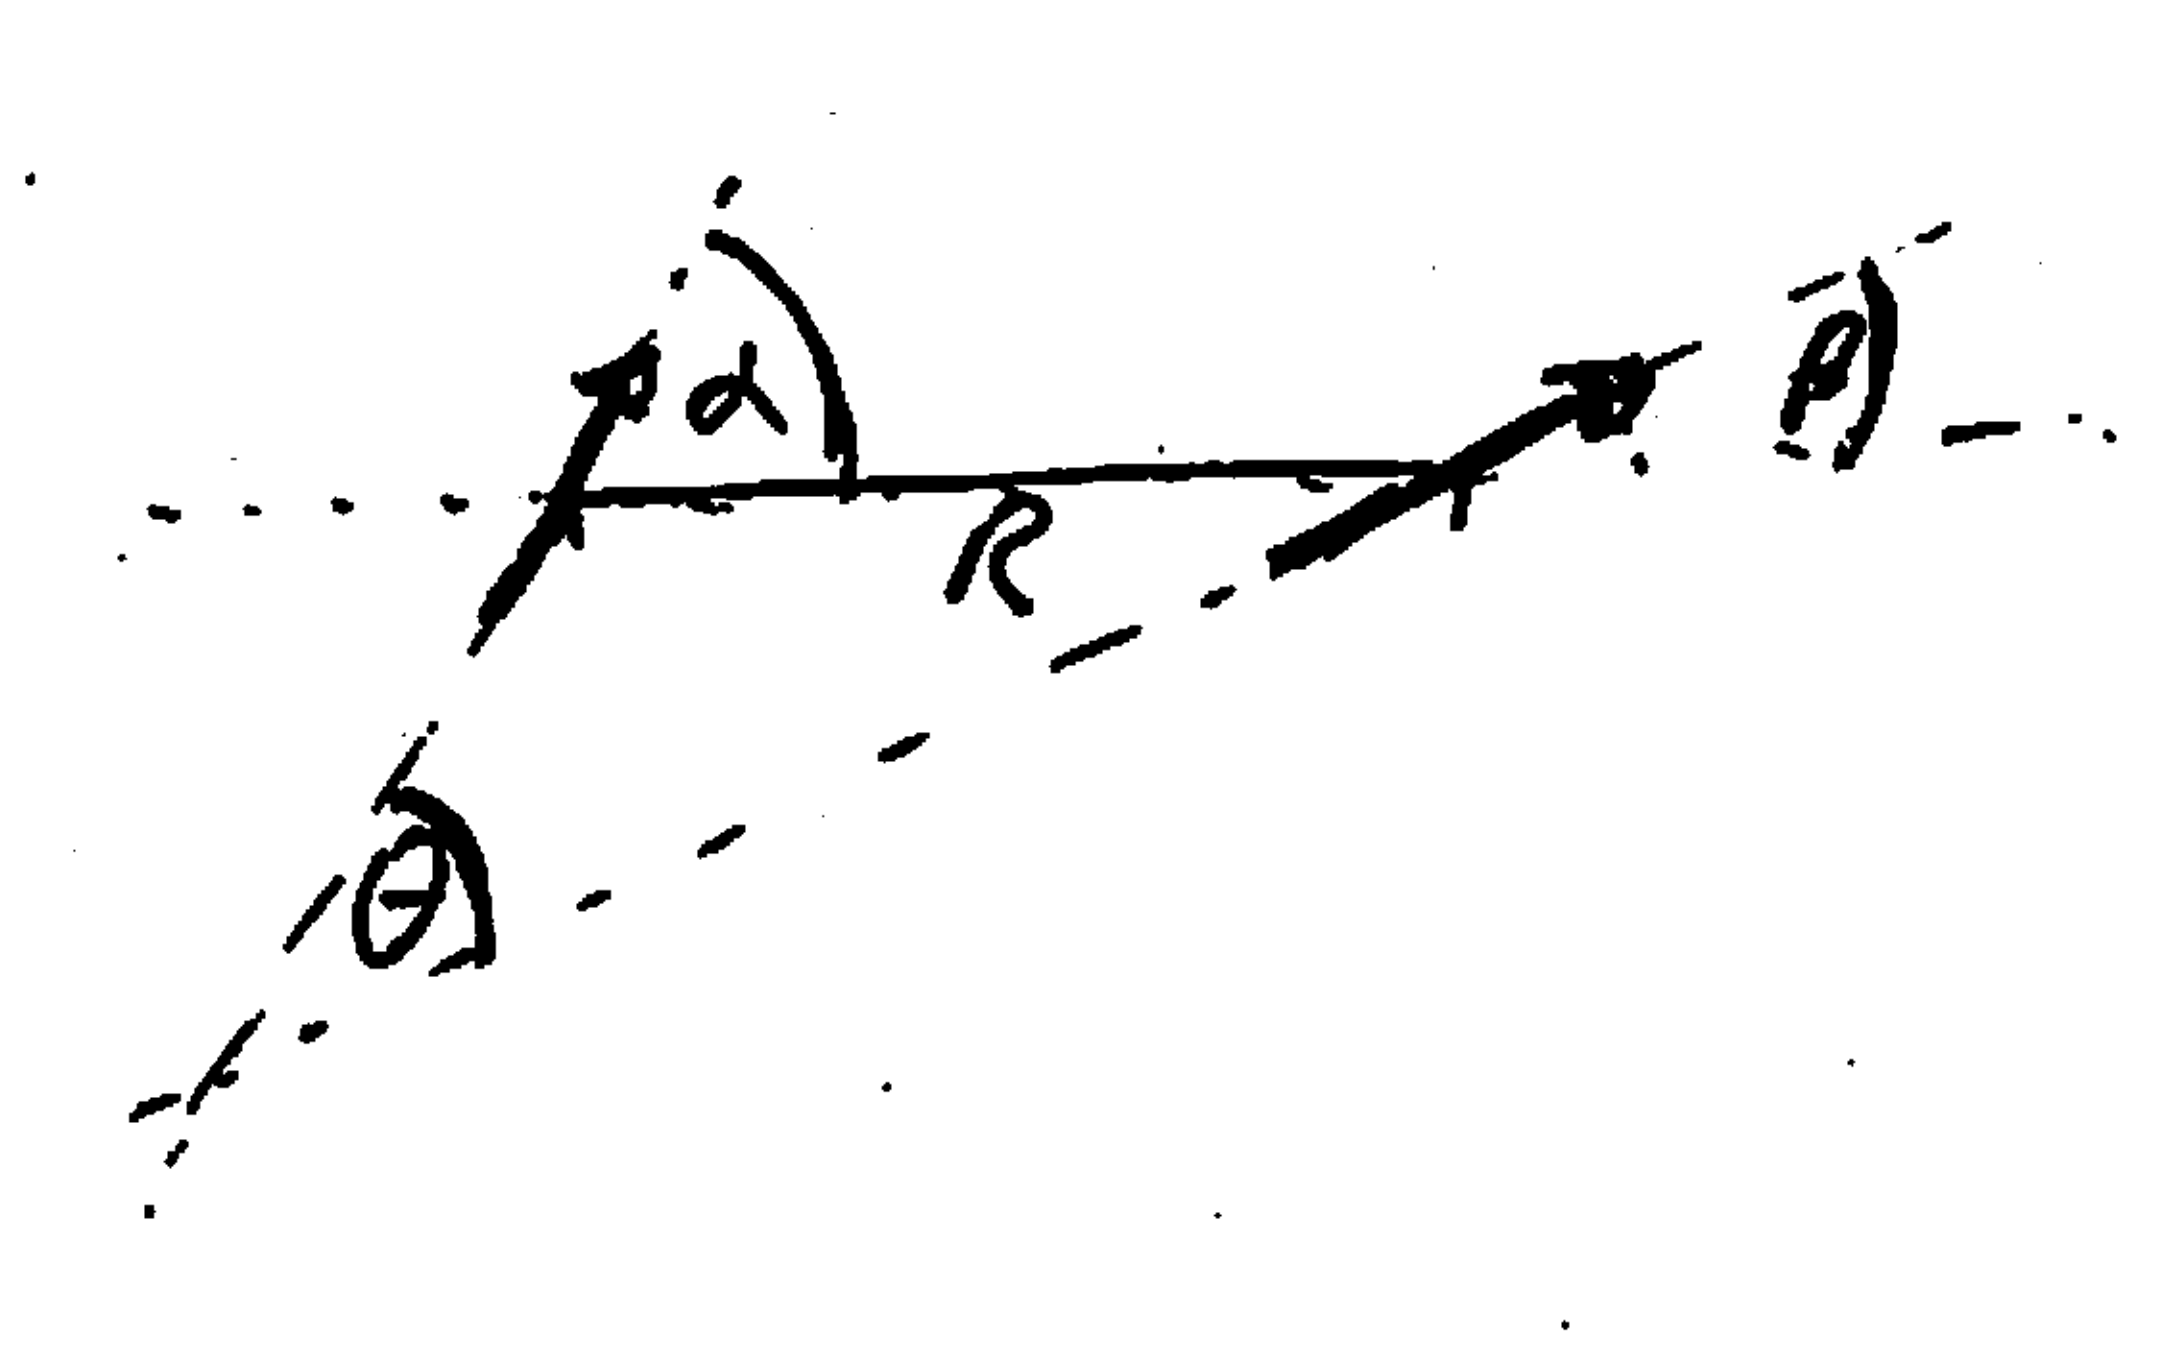
\includegraphics[width=\textwidth]{\currfiledir/angles.png}
   \inputtikz{\currfiledir/angles}

\caption{Sketch showing 
the angles used to calculate the coupling factor $\kappa$}
\end{marginfigure}

A similar coupling term also exist for the non-resonant coupling\footcite{knoester-book}
\begin{equation}
\hat{H}_{non-res} = J \left(  \ket{11}\bra{00} + \ket{00}\bra{11}  \right)
\end{equation}
but this can be ignored, as it is non-resonant. Altogether, the Hamilton operator reads in matrix form
\begin{equation}
\hat{H} = \begin{pmatrix}
0   					& \mu_a 						&	\mu_b						& 		J 		\\
\mu_a^\star	& \hbar \omega_a		&	J								& \mu_b	\\
\mu_b^\star  &  J^\star					& \hbar \omega_b		& \mu_a	\\
J^\star				& \mu_b^\star			& \mu_a^\star			& \hbar (\omega_a + \omega_b) \\
\end{pmatrix} \quad .
\end{equation}
When we ignore the double-excited state $\bra{11}$, the essence in contained in the center $2 \times 2$ matrix which we discussed already in the preceding section.

When $\ket{\psi}$ is a linear combination of $\ket{01}$ and $\ket{10}$, then also the transition dipole moment from $\ket{00}$ to $\ket{\psi}$ is a linear combination of $\mu_a$ and $\mu_b$ with the same weights. When $J \gg |E_a - E_b| / 2$ then we get
\begin{equation}
 \boldsymbol{\mu}_{\pm} = \sqrt{1/2} \, \left( \boldsymbol{\mu}_a \pm  \boldsymbol{\mu}_b  \right)  \quad .
\end{equation}
The brightness of the absorption line is for identical molecules, i.e. $\mu = \mu_a = \mu_b$
\begin{equation}
 I \propto |\boldsymbol{\mu}_{\pm}|^2 = (1/2) \, \left| \boldsymbol{\mu}_a \pm  \boldsymbol{\mu}_b  \right|^2 =  \left( 1 \pm \cos \theta \right) \, \left| \boldsymbol{\mu}   \right| ^2  \quad ,
\end{equation}
where $\theta$ is as above the angle between the transition dipole moments. The same relation hold for the radiative rate.

The spectroscopic signature of coherent coupling between two molecules is thus a splitting of the absorption line into two lines, separated by twice the coupling energy $J$. The sum of the line amplitudes remains unchanged, but in some cases (H- and J-aggregates, see below) one transition will take the whole amplitude and the other remains dark. In these cases, no splitting but a shift of the absorption line is observed. The coupling vanishes when both dipoles are oriented perpendicular to each other ($\theta = 90^\circ$)


\section{H- and J-aggregates}

\begin{marginfigure}
%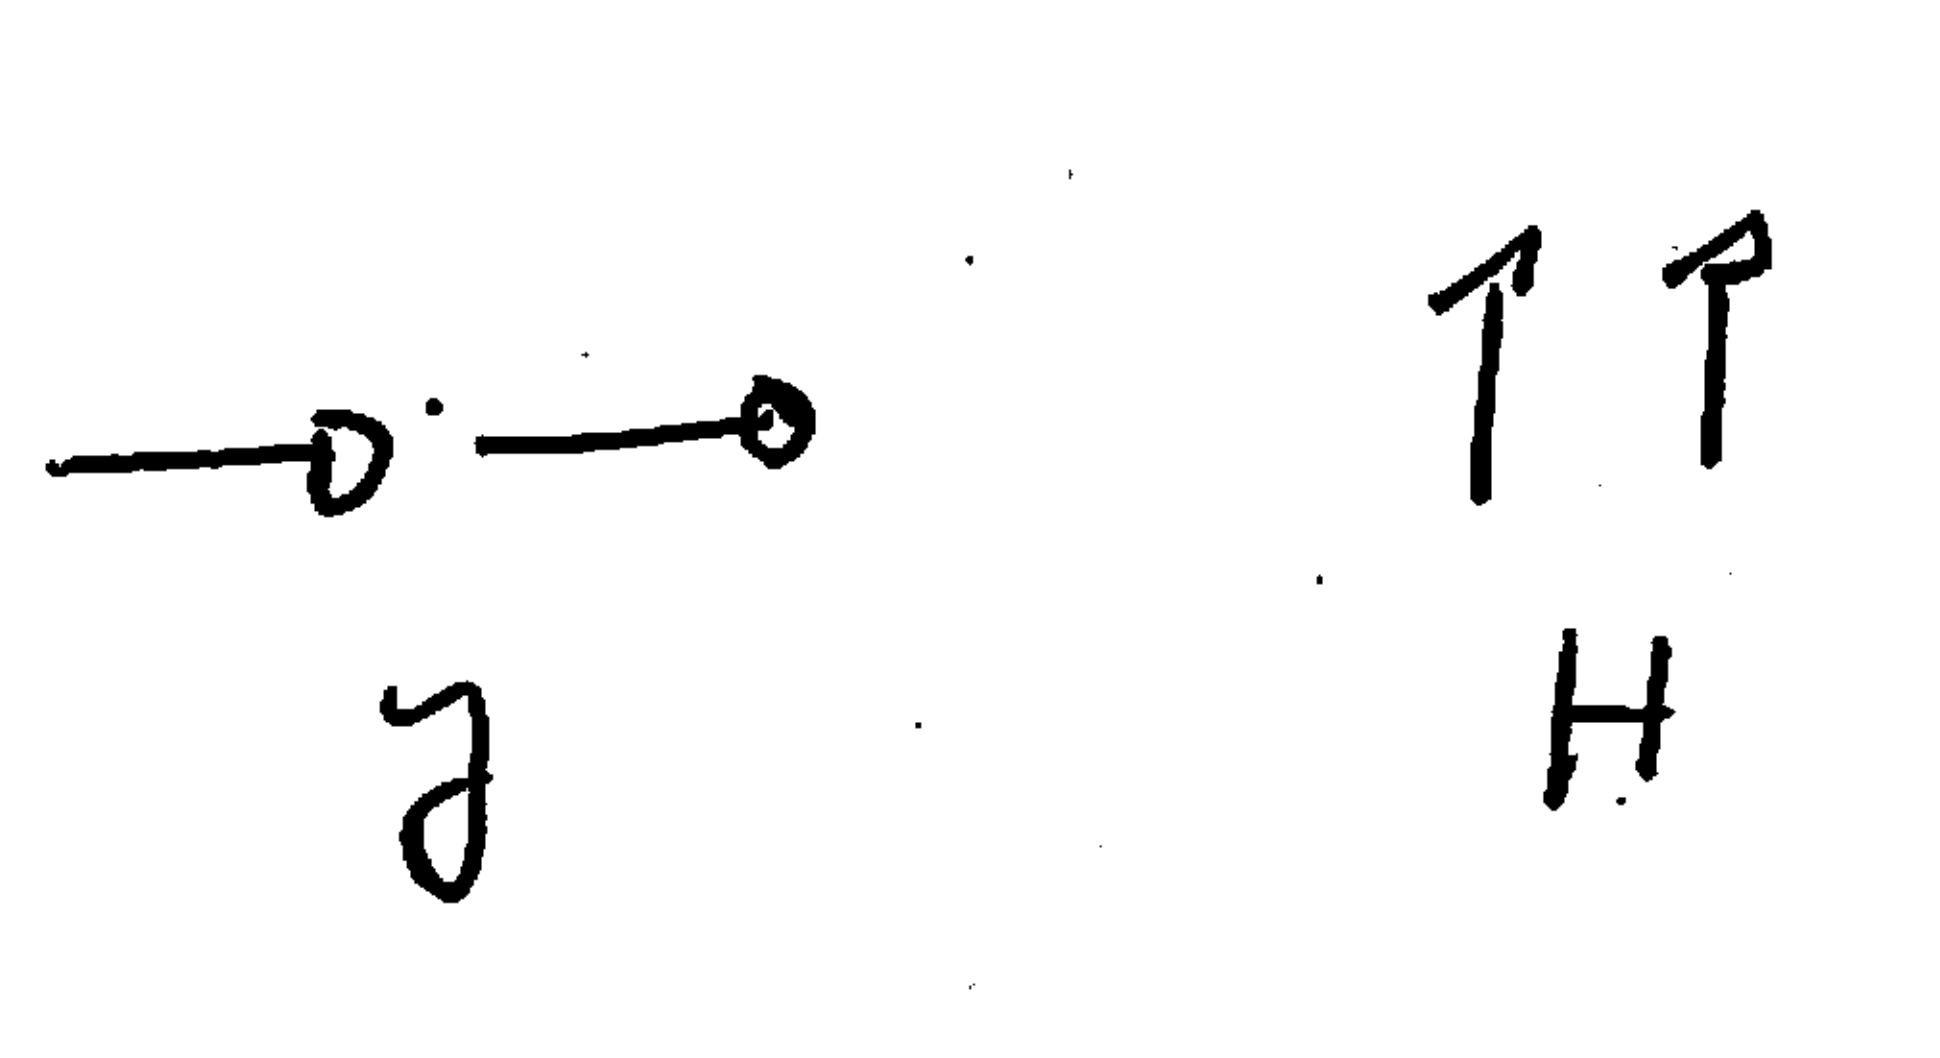
\includegraphics[width=\textwidth]{\currfiledir/aggregates.png}
   \inputtikz{\currfiledir/jh}

\caption{J- and H aggregates.}
\end{marginfigure}


Two important limiting cases are the H- and J-aggregates\footcite[chapters 2.1.4.3, 2.2.5.3]{KoehlerBaessler2015} In a J-aggregate, the dipoles are oriented parallel and head-to-tail, i.e. $\alpha = \beta = \theta = 0$ and therefore $\kappa = -2$. A negative $\kappa$ implies that the coupling constant $J$ is negative. The state $\Psi_+$, which carries all the oscillator strength, has the energy $E_+ = (E_a + E_b) / 2 + J$, which is lower than the average energy of the uncoupled states. The absorption line thus shifts to the red. The same hold for the fluorescence emission spectrum.

In an H-aggregate, the dipoles orient also parallel, but side-to-side, i.e.  $\alpha = \beta = 90^\circ$ and $\theta = 0$. In this case is $\kappa =1$ and $J$ positive. The absorption line shifts to the blue upon formation of aggregates, as again the  $\Psi_+$ state gets all the oscillator strength. However, as fluorescence emission is slow compared to other relaxation processes, this high energy state does not emit light. In emission, H-aggregates appear dark.

The width of the absorption line of a dye at room temperature is determined by dephasing, i.e., fluctuations in the environment that are fast compared to the lifetime of the excited state, and by static differences in the environment of different chromophores. The spectral position of the absorption line in a molecular aggregate is the average of two single chromophore transitions. As in the propagation of uncertainties in an experiment, the width of the new distribution, generated as the average over two values from the old distribution, is reduced by a factor of $\sqrt{2}$. This holds more generally\footcite{Knapp1984}, so that an aggregate of $N$ chromophores is expected to have a spectral line width reduced\sidenote{This is the same physics as motional narrowing in NMR.} by $\sqrt{N}$.




%\begin{tabular}{llll}
%$\theta$	&	$0^\circ$ & $90^\circ$ & $0^\circ$  \\
%$\alpha$ & $0^\circ$ & $0^\circ$ & $90^\circ$  \\
%$\beta$ & $0^\circ$ & $90^\circ$ & $90^\circ$  \\
%$\kappa$  & $-2	$	& 	 $	0	$				& $1$   \\
%\end{tabular}




\printbibliography[segment=\therefsegment,heading=subbibliography]


%-------


\part{Single Molecule Spectroscopy}



\chapter{Fluorescence correlation spectroscopy -- FCS}


\textit{Bestimmen sie die Konzentration und den Diffusionskoeffizienten / Gyrationsradius des Nanoobjekts, CdSe NC, R6G}


\textit{Add-on: berechnen sie die AC aus der Zeitspur}


\section{Experiment}

The data sets contain absorption spectra as measured with a commercial UV/VIS spectrometer. Determine the absorption cross section of each species and compare to its geometrical size. Determine also the oscillator strength, the transition dipole moment, and the transition matrix element.

assuming that almost all atoms are in the ground state ($N_2 \ll N_1$). Note that this absorption cross section $\sigma$ is not a function of angular frequency $\omega$ anymore, but an spectral integrated cross section assuming a black body spectrum.\sidenote{really ???}





\printbibliography[segment=\therefsegment,heading=subbibliography]



\chapter{Fluorescence anisotropy \& rotational diffusion}

\textit{Küvette und TCSPC
}
\section{Experiment}

The data sets contain absorption spectra as measured with a commercial UV/VIS spectrometer. Determine the absorption cross section of each species and compare to its geometrical size. Determine also the oscillator strength, the transition dipole moment, and the transition matrix element.

assuming that almost all atoms are in the ground state ($N_2 \ll N_1$). Note that this absorption cross section $\sigma$ is not a function of angular frequency $\omega$ anymore, but an spectral integrated cross section assuming a black body spectrum.\sidenote{really ???}





\printbibliography[segment=\therefsegment,heading=subbibliography]



\chapter{k-space imaging}


\textit{bestimmen sie die Orientierung des Dipols, CdSe NC, R6G
}
\section{Experiment}

The data sets contain absorption spectra as measured with a commercial UV/VIS spectrometer. Determine the absorption cross section of each species and compare to its geometrical size. Determine also the oscillator strength, the transition dipole moment, and the transition matrix element.

assuming that almost all atoms are in the ground state ($N_2 \ll N_1$). Note that this absorption cross section $\sigma$ is not a function of angular frequency $\omega$ anymore, but an spectral integrated cross section assuming a black body spectrum.\sidenote{really ???}





\printbibliography[segment=\therefsegment,heading=subbibliography]



\chapter{Blinking \& Bleaching}



\textit{Ändert sich die strahlende oder die nicht-strahlende Rate, CdSe NC
}
\section{Experiment}

The data sets contain absorption spectra as measured with a commercial UV/VIS spectrometer. Determine the absorption cross section of each species and compare to its geometrical size. Determine also the oscillator strength, the transition dipole moment, and the transition matrix element.

assuming that almost all atoms are in the ground state ($N_2 \ll N_1$). Note that this absorption cross section $\sigma$ is not a function of angular frequency $\omega$ anymore, but an spectral integrated cross section assuming a black body spectrum.\sidenote{really ???}





\printbibliography[segment=\therefsegment,heading=subbibliography]



\chapter{Photon Antibunching}



\textit{Modellieren und bestimmen sie g(2), TDI
}
\section{Experiment}

The data sets contain absorption spectra as measured with a commercial UV/VIS spectrometer. Determine the absorption cross section of each species and compare to its geometrical size. Determine also the oscillator strength, the transition dipole moment, and the transition matrix element.

assuming that almost all atoms are in the ground state ($N_2 \ll N_1$). Note that this absorption cross section $\sigma$ is not a function of angular frequency $\omega$ anymore, but an spectral integrated cross section assuming a black body spectrum.\sidenote{really ???}





\printbibliography[segment=\therefsegment,heading=subbibliography]



\chapter{Förster Resonant Energy Transfer -- FRET}



\section{Experiment}

\textit{spektral, fl. Lifetime, ensemble, JK dyade
}
\textit{Wie groß ist der Förster-Radius des Paares? Wie groß ist die Transfer-Effizient in dieser Dyade?
}


\section{Forester Theory (FRET)\protect\footnote{Parson, ch. 7.2, Simon Biberger}} 


One way for an excited molecule to reach the ground state is by transferring this energy to another molecule. This is called resonance energy transfer.
At the beginning, two adjacent but non-interacting molecules 1 and 2 shall be considered. Their Hamiltonian operator is then
\begin{equation*}
    H = H_1 + H_2
\end{equation*}
and the associated overall wave function for the ground state is the product of the two individual wave functions.
\begin{equation*}
    \Psi_{Ges} = \Phi_{1a} \chi_{1a}\cdot \Phi_{2a} \chi_{2a}
\end{equation*}
If now one of the two molecules is excited, the total wave function becomes closed:
\begin{equation*}
    \Psi_{Ges} = C_1 \Phi_{1b} \chi_{1b}\cdot \Phi_{2a} \chi_{2a} + C_2 \Phi_{1a} \chi_{1a}\cdot \Phi_{2b} \chi_{2b}
\end{equation*}

The factors $C_1$ and $C_2$ represent the probability that the molecule is excited. Here $|C_1|^2 + |C_2|^2 = 1$.
In Förster theory, an interaction between the molecules is now allowed and the Hamilton operator is
\begin{equation*}
    H_{Ges} = H_1 + H_2 + H_{21}
\end{equation*}
If one starts at the time t\,=\,0 with $C_1$\,=\,1 and $C_2$\,=\,0, $C_2$ can be determined via time-dependent perturbation theory:
\begin{equation}
    C_2 = H_{21} \frac{1 - exp \left[\frac{i(E_2 - E_1)t}{\hbar} \right] } {E_2 - E_1}
    \label{c2}
\end{equation}
From equation \ref{c2} the resonance condition for the energy difference between molecule 1 and 2 can be derived immediately. $C_2$ has only a significant amount if the energy difference is as small as possible.


\begin{figure}
\label{Resonance}
\center
    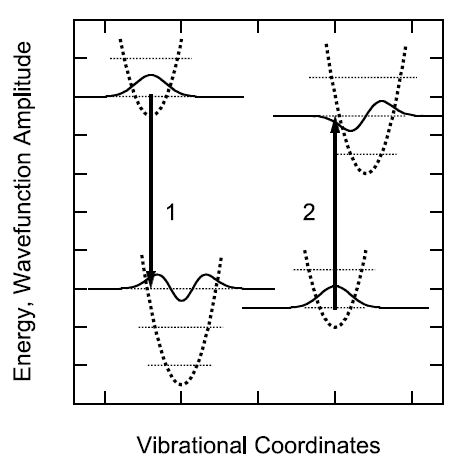
\includegraphics[width = 0.7 \textwidth]{\currfiledir/FRET.JPG}
    \caption{The resonance-energy transfer requires coupled vibronic transitions up and down. The energy lost by molecule 1 must be absorbed by molecule 2, so that the energy is maintained overall. In addition, the associated Frank-Condon factors for the transitions must be non-zero.}
\end{figure}

The total rate of energy transfer can be determined using Fermi's Golden Rule:
\begin{equation*}
    k_{rt} = \frac{2\pi}{\hbar} \cdot \int_{-\infty}^{+\infty} |H_{21}|^2 \rho_{s2}(E_1) \rho_{s1}(E_1) dE_1,
\end{equation*}
where $\rho_{si}$ denotes the state densities of molecule 1 and 2

\section{FRET on single molecules for distance measurement\protect\footnote{Parson, sections 7.2 and 7.3}} 

The strong distance dependence of FRET is used to
the relative spatial position of marker fluorophores
for example in proteins.

The transfer of energy from one excited fluorophore to another can be described with the theory of Förster resonance energy transfer. The energy transfer takes place without radiation via a dipole-dipole interaction. The rate constant $k_{rt}$ for this transition is defined as follows:
\begin{equation}
    k_{rt}=\left( \frac{9000 ln(10)\kappa^2c^4\Phi}{128\pi^5n^4N_A\tau} \right) |R_{21}|^{-6}J ,
\end{equation}
where $\kappa$ is the orientation factor, $\Phi$ and $\tau$ the quantum yield and lifetime of the donor, $R_{21}$ the distance between donor and acceptor, and J is an overlap integral between the absorption and emission spectrum of the fluorophores involved. The orientation factor $\kappa$ indicates the orientation of the two interacting partners assumed to be dipoles and can take values between $-2$ and $2$ (see Fig. \ref{KappaFactor}). 

\begin{figure}
\label{KappaFaktor}
\center
    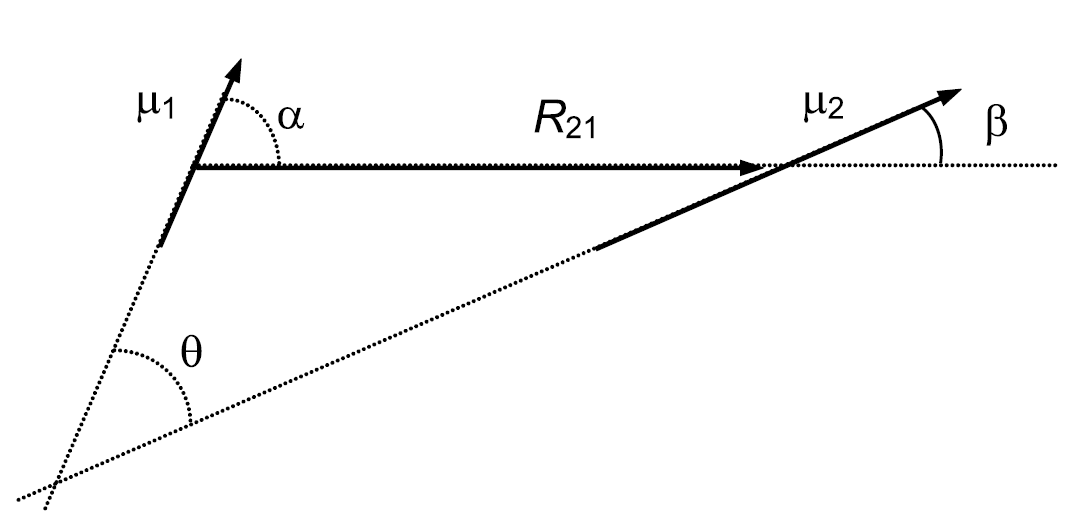
\includegraphics[width = 0.5 \textwidth]{\currfiledir/FretKappa.png}
    \caption{Sketch for the position of the angles and the distance of the dipoles. The orientation factor $\kappa$ is described by: $\kappa=\cos(\theta)-3 \cos (\alpha)\cos (\beta)$}
\end{figure}
The equation for the rate constant is also often given in the shortened form
\begin{equation}
\label{eq:fret}
    k_{rt}=\tau^{-1}(|R_{21}|/R_0)^{-6}
\end{equation}
with the forest ranger radius $R_0$. This indicates the distance at which the efficiency\footnote{The efficiency $E$ is defined as $E=\frac{1}{1+(r/R_0)^6}$ } of the energy transfer is 50\%.\par
To determine the distance between two molecules using Fret, the rate constant $k_{rt}$ must first be calculated from the fluorescence yields in the presence $\Phi$ and absence of the acceptor $\Phi_q$ using the following formula 
\[ \frac{\Phi}{\Phi_q}=1+k_{rt}\tau .\]
If the product of $k_{rt}\tau$ and the forester radius is known, the distance $|R_{21}|$ can be calculated from equation \ref{eq:fret}.




\printbibliography[segment=\therefsegment,heading=subbibliography]


%-------


\part{Two Level Systems}



\chapter{Overview TLS}





1.	Rabi Oszillationen

2.	(perturbed) Free induction decay

3.	Ramsey fringes

4.	Double resonance spectroscopy

5.	Frequency modulation / Kador

6.	Quantum beats

7.	Strong coupling 

8.	Pump-probe spectroscopy (?)

9.	2D spectroscopy, Feynman diag.





Wir beginnenn die kohärente Spektroskopie  mit ein paar
Grundlagen (und einem neuen Buch).

\section{8.1. Wdh. Störungsrechnung, Fermis Goldene Regel und
Einstein-Koeffizienten\protect\footnote{Rand, Kap. 3.2 und 3.5}\hfill w} 

Das haben wir schon gemacht. Freunden sie sich mit der
Notation von Stephen Rand an.

\section{8.2. Störungsrechnung vs. Exakte Lösung (Rabi)\protect\footnote{Rand, Kap. 3.3 \newline Hamm 2005, Kap. 1 \newline Christoph Schnupfhagn}\hfill *} 

Verstehen sie die Grenzen der Störungsrechung und den
Unterschied zum exakten Rabi-Formalismus. \footnote{Warum vergleicht Rand das Ergebnis der Störungsrechnung mit Dämpfung mit der Lösung von Rabi ohne Dämpfung? Vergleicht man die Ergebnisse jeweils ohne Dämpfung, sind diese bis auf den Vorfaktor vor der Oszillation sehr ähnlich.}

Mit dem Störungsansatz für den Hamiltonoperator, welcher bereits in Kapitel \ref{sec:stoerungstheorie} eingeführt wurde, lassen sich die Differentialgleichungen für die Zeitentwicklung der Faktoren $C_{1}$ und $C_{2}$ herleiten. In der \emph{rotating wave approximation} (Vernachlässigung der Terme mit $\omega_{0} + \omega$) lauten diese:
\begin{align}
    \dot{C_{2}} & = \frac{i \Omega}{2} e^{i (\omega_{0} - \omega) t} C_{1} - \frac{1}{2} \gamma_{2} C_{2} \label{eq:rabi1} \\
    \dot{C_{1}} & = \frac{i \Omega^{\ast}}{2} e^{-i (\omega_{0} - \omega) t} C_{2} - \frac{1}{2} \gamma_{1} C_{1} \label{eq:rabi2}
\end{align}
Dabei ist $\Omega = \vec{\mu}_{21} \cdot \vec{E}_{0} / \hbar$ und $\omega_{0}$ die Differenzfrequenz der Energieniveaus 1 und 2. Die zweiten Summanden werden jeweils phänomenologisch hinzugefügt, um der spontanen Relaxation der Zustände Rechnung zu tragen. Im Folgenden wird jedoch $\gamma_{1} = \gamma_{2} = 0$ angenommen.

Bisher wurde das obige System zweier Differentialgleichungen für kleine Zeiten genähert. Aufgrund der Anfangsbedingungen $C_{1}(0) = 1$ und $C_{2}(0) = 0$ gilt dann
\begin{align}
    \dot{C_{2}} & = \frac{i \Omega}{2} e^{i (\omega_{0} - \omega) t} C_{1} \\
    \dot{C_{1}} & = 0.
\end{align}
Die Wahrscheinlichkeit, dass sich das Molekül nach der Zeit $t$ im angeregten Zustand befindet, ist dann gegeben durch
\begin{equation}
    \vert C_{2}(t) \vert^{2} = \left[ \frac{\Omega}{2} \frac{\sin((\omega_{0} - \omega) t/2)}{(\omega_{0} - \omega)/2} \right]^{2}
    \label{eq:c2-approx}
\end{equation}
und oszilliert somit in der Zeit. Die Lösung divergiert allerdings für $\omega_{0} \rightarrow \omega$, d.h.\ bei der Resonanz. Da aus Gründen der Normierung immer $\vert C_{2}(t) \vert^{2} \leq 1$ gelten muss, ist diese Lösung nicht physikalisch.

Gleichungen \ref{eq:rabi1} und \ref{eq:rabi2} können jedoch auch exakt gelöst werden für den Fall $\gamma_{1} = \gamma_{2} = 0$, was als Rabi-Formalismus bezeichnet wird. Daraus ergibt sich die Besetzungswahrscheinlichkeit
\begin{equation}
    \vert C_{2}(t) \vert^{2} = \left[ \frac{\Omega}{2} \frac{\sin(\Omega_{R} t/2)}{\Omega_{R}/2} \right]^{2}
\end{equation}
mit der Rabi-Flopping-Frequenz $\Omega_{R} = [ \Delta^{2} + \Omega^{2} ]^{1/2}$ und $\Delta = \omega_{0} - \omega$. $\vert C_{2}(t) \vert^{2}$ ist für den Resonanzfall $\Delta = 0$ in Abbildung \ref{fig:rabi} eingezeichnet. Es ist zu erkennen, dass das Molekül periodisch zwischen angeregtem und Grundzustand wechselt (\emph{Rabi Flopping}) und somit eine periodische Besetzungsinversion erreicht werden kann. Die Lösung von Rabi zeigt keine Divergenz mehr im Vergleich zu Gleichung \ref{eq:c2-approx}.

\begin{figure}
    \centering
    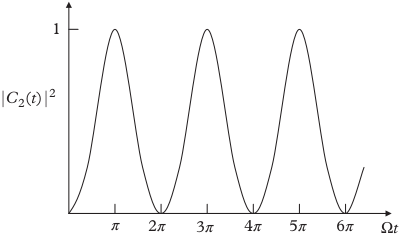
\includegraphics[width = 0.7 \textwidth]{\currfiledir/Rabi.png}
    \caption{Lösung von Rabi im Resonanzfall $\Delta = 0$. Das Molekül wechselt periodisch zwischen angeregtem und Grundzustand.}
    \label{fig:rabi}
\end{figure}

\section{8.3. Dichte-Matrix\protect\footnote{Rand,  Kap. 3.6 \newline Parson, Kap. 10.2 \newline Hamm 2005, Kap. 1}\hfill **} 

Die Dichte-Matrix ist wichtig, um inkohärente Zustände zu
beschreiben, kommt in der QM aber oft zu kurz. \footnote{Warum kann man ein Ensemble von Teilchen nicht durch eine einzelne Wellenfunktion beschreiben, sondern nur durch eine Summe von Dichtematritzen?}
\footnote{Ich habe das so verstanden, dass ein reiner Zustand eine köhärente Superposition einzelner Zustände und damit Wellenfunktionen ist. Hat dieser Begriff der Kohärenz etwas mit dem aus der Optik zu tun?}

\section{8.4. Optische Bloch-Gleichungen\protect\footnote{Rand, Kap. 3.8, Simon Biberger}\hfill ***} 

\textit{Man kann die Wechselwirkung von Licht mit einem
Zwei-Niveau-System auf Kreisel-Physik abbilden.}
\footnote{Was versteht man unter inkohärentem Pumpen?}
\footnote{Was genau kann man sich unter dephasing vorstellen?}
Um den Hermiteschen Charakter des Hamilton-Operators zu erhalten, muss beim Beachten von Zerfallstermen die Bewegungsgleichung folgendermaßen modifiziert werden.
\begin{align}
    i\hbar \dot{\hat{\rho}} =& [\hat{H},\hat{\rho}] + Relaxationsterme \notag\\
    =& [\hat{H},\hat{\rho}] \pm i\hbar\Lambda \pm i\hbar\gamma \hat{\rho} - i\hbar \Gamma \hat{\rho}
\end{align}
Der erste Term berücksichtigt die Abnahme durch inkohärentes Pumpen, der zweite die strahlende und nicht-strahlende Populations-Relaxation. Der letzte beachtet das dephasing. %dem Verlust der genauen Information über die zeitliche Entwicklung der Signale 

Unter bestimmten Bedingungen können die Dichte-Matrix-Bewegungsgleichungen in eine praktische Form übergeführt werden, die als optische Bloch-Gleichungen bekannt sind, welche eine ähnliche Form wie die Kreisel-Präzession besitzen. Die einfachste Form der Bloch-Gleichungen beschreibt ein Zwei-Niveau-System und wird Vektor-Modell genannt.\\

Mithilfe der Rotating-Wave-Approximation (RWA) und der slowly varying envelope approxiamtion (SVEA) erhält man
\begin{align}
    V_{21}=& -\frac{1}{2}\mu_{21}E_0e^{-i\omega t} \label{Bloch1}\\
    \rho_{21} =& \tilde{\rho}_{21}e^{-i\omega t} \label{Bloch2}.
\end{align}
$\tilde{\rho}_{21}$ beschreibt hier die langsam variierende Amplitude des Matrixelemente, welche proportional zur Amplitude der Ladungs-Oszillation bei der bestimmten optischen Frequenz ist.\\
Mit den Gleichungen \ref{Bloch1} und \ref{Bloch2} erhält man für die Zeitentwicklung von $\tilde{\rho}_{21}$:
\begin{equation}
    \left( \frac{d}{dt} + i\Delta + \Gamma\right)\tilde{\rho}_{21}=-\frac{i}{2}\Omega(\rho_{22}-\rho_{11}).
\end{equation}
Dabei gilt $\Delta$= $\omega_0 - \omega$ und $\Omega$ = $\frac{\mu_{21}E_0}{\hbar}$.\\
Damit lassen sich drei Komponenten eines 3-dim. Vektors definieren.
\begin{align}
    R_1 =& \tilde{\rho}_{21} + \tilde{\rho}_{12}  \notag \\
    R_2 =& i(\tilde{\rho}_{21}-\tilde{\rho}_{12})\\
    R_3 =& \rho_{22} -\rho_{11} \notag
 \end{align}
 \begin{equation}
     \bar{R} = R_1\tilde{e}_1 + R_2\tilde{e}_2 + R_3\tilde{e}_3
 \end{equation}
 Für die Zeitentwicklung der drei Komponenten erhält man mit $\Gamma$ = $\frac{1}{T}$:
 \begin{align}
    \dot{R_1} =& -\Delta R_2 - \frac{1}{T}R_1  \notag \\
    \dot{R_2} =& \Delta R_1 - \frac{1}{T}R_2 + \Omega R_3 \label{Bloch3}\\
    \dot{R_3} =& - \frac{1}{T}R_3 - \Omega R_2 \notag
 \end{align}
 Die Gleichungen \ref{Bloch3} werden optische Bloch-Gleichungen genannt. Kompakter lassen sich die drei Gleichungen mit
 \begin{equation}
     \dot{\bar{R}} = -\frac{1}{T}\bar{R} + \bar{\beta} \times \bar{R}
 \end{equation}
schreiben, wobei $\bar{\beta}$ = $\Omega \hat{e}_1$ + $\Delta \hat{e}_3$ ist.\\
Die Bewegung des Bloch-Vektors ist in Abbildung \ref{fig:Bloch} zu sehen. Für die gezeigte Orientierung von $\bar{\beta}$ ist das detuning positiv.
\begin{figure} [h]
    \centering
    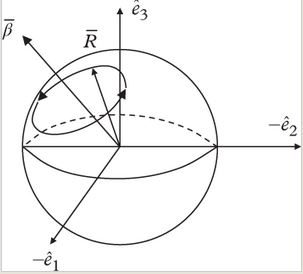
\includegraphics[width = 0.7 \textwidth]{\currfiledir/Bloch.JPG}
    \caption{Präzession des Bloch-Vektors $\bar{R}$ um ein effektives Feld $\bar{\beta}$.}
    \label{fig:Bloch}
\end{figure}
\section{8.5. Polarization und abgestrahlte Felder\protect\footnote{Rand, Kap. 3.9}\hfill **} 

Wie kommt es, dass man am Ende etwas detektieren kann? \footnote{Die Lösung der Wellengleichung liefert ein elektrisches Feld, dessen Betrag proportional zur Länge der Probe ist. Eigentlich sollte dies aber doch das Pendant zum Lambert-Beerschen Gesetz sein, also eher einen exponentiellen Zusammenhang mit der Länge aufweisen?}

\section{8.6. Absorption in der Dichte-Matrix-Darstellung\protect\footnote{XXX ???}\hfill *} 

Das Optische Theorem hilft zu verstehen, warum in einem
Transmissionsexperiment am Ende Licht fehlt, und wie das mit
der Dichtematrix zusammenhängt.



\section{ 9. Effekte der Bloch-Gleichungen / NMR mit Licht} 

Wir betreiben Kreisel-Physik  mit Licht anhand von einigen
klassischen Beispielen

\section{9.1. Rabi-Oszillationen\protect\footnote{Rand, Kap. 4.1, Simon Biberger}\hfill ***} 

\textit{Das Zwei-Niveau-System oszilliert entweder als Funktion der
Zeit oder der 'pulse area' zwischen Grund- und angeregtem
Zustand.}\\
Betrachtet man ein Atom, das plötzlich Licht ausgesetzt ist, welches resonant mit einem Übergang aus dem Grundzustand ist. So kann es zu einem kohärenten transienten Phänomen kommen, der Nutation. Die Nutation beschreibt den Aufbau einer Polarisation, welche durch die Anwesenheit eines optischen Feldes verursacht wird.\\
Da die Rabi-Oszillationen in Bezug auf Populationszerfälle schnelle Prozesse sind, vereinfachen sich die Bloch-Gleichungen zu:
\begin{align}
    \dot{R_1} =& -\Delta R_2  \notag \\
    \dot{R_2} =& \Delta R_1 + \Omega R_3 \label{Rabi}\\
    \dot{R_3} =& - \Omega R_2 \notag
 \end{align}
Diese Gleichungen lassen sich bei Mitnahme eines möglichen Doppler-Shifts ($v_z$) und mit einer Anfangsverteilung der Population $R_3$(0) lösen.
\begin{align}
    R_1(t) =& \frac{\Omega \Delta}{\Omega_R^2}R_3(0)\cdot cos(\Omega_Rt-1) \notag \\
    R_2(t) =& \frac{\Omega}{\Omega_R}R_3(0)\cdot sin(\Omega_Rt) \label{Rabi2}\\
    R_3(t) =& R_3(0)\cdot \left[1+\frac{\Omega^2}{\Omega_R^2}\cdot 
    cos(\Omega_Rt-1)\right] \notag
\end{align}
Dabei ist $\Omega_R^2$ = $\Delta^2 + \Omega^2$, $\Delta = \omega_0-\omega-kv_z$ und $\Omega = \mu_{21}E_{12}/\hbar$.\\
Der Betrag des Bloch-Vektors bleibt über die betrachtete Zeit konstant. Er präzediert um den Vektor $\bar{\beta}$ mit der Frequenz $\Omega_R$.
Für den Resonanzfall $\Delta = 0$ kommt es zum Rabi-flopping. Dabei springt  $\bar{\beta} = \Omega \hat{e}_1$ auf $\bar{\beta} = -\Omega \hat{e}_1$. Das Atom oszilliert also zwischen dem angeregten und Grundzustand unter dem Einfluss eines treibenden Feldes.\\
Die Rabi-Oszillationen können über zwei Methoden gemessen werden. Entweder betrachtet man die Zeitentwicklung der Fluoreszenz bei einem festen treibenden Feld oder die Transmissionsänderung während der Variation der treibenden Feldes.
\begin{figure} [h]
    \centering
    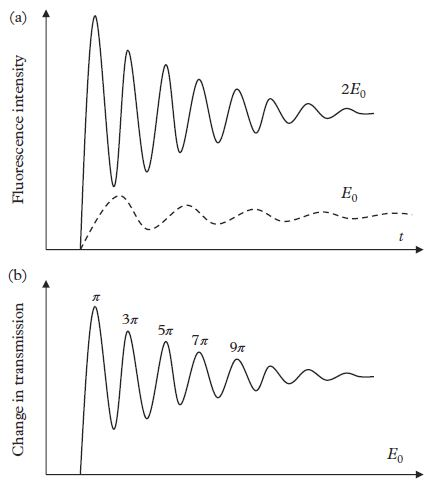
\includegraphics[width = 0.7 \textwidth]{\currfiledir/Rabi1.JPG}
    \caption{Rabi-Oszillationen in (a) transienter Fluoreszenz und (b) differentielle Transmissionsmessung.}
    \label{fig:Rabi}
\end{figure}

\section{9.2. Free Induction Decay\protect\footnote{Rand, Kap. 4.2}\hfill **} 

Nach dem Ausschalten des Lasers wird noch ein Feld
abgestrahlt.

\section{9.3. Photon Echo\protect\footnote{Rand, Kap. 4.3}\hfill ***} 

Mehrere Lichtpulse wechselwirken mit einem inhomogenen
Ensemble von Atomen / Fluorophoren. Nachdem alle Pulse
vorbei sind wird trotzdem noch ein Feld emittiert. Dies ist
eine elegante Methode, um die Inhomogenität eines Ensembles
zum umgehen.
 
 

%-------


\part{Nonlinear Spectroscopy}



\chapter{Overview NLO}




\textbf{SHG, phase matching
}
SHG efficiency as function of angle / temperature
determine crystal orientation / model data from crystal orientation

\textbf{FWM}
Model data

\textbf{Pulse shaper:} linear + nonlinear, CEP and without

Pump-probe, 2D ?

THG

Frog etc.



Wir untersuchen systhematisch die kohärente Wechselwirkung
von mehreren Lichtpulsen mit einer Probe. Mir gefällt hier
das Skript von P.~Hamm am besten.

\section{10.1. Wdh. Liouville-Gleichung\protect\footnote{Hamm 2005, Kap. 1}\hfill w} 

Das ist  die Schrödinger-Gleichung für Dichte-Matrix, inkl.
Zerfallsprozessen. Eigentlich nur eine elegante
Schreibweise.

Unter Verwendung gewöhnlicher Zustände findet man

\begin{equation}
    \frac{\partial}{\partial t}|\psi\rangle = -\frac{i}{\hbar}|\psi\rangle
\end{equation}

Beschreibt man das System nicht mit $|\psi\rangle$, sondern mit der Dichtematrix $\rho = |\psi\rangle\langle\psi|$, so findet man für deren Zeitentwicklung die Louville-Gleichung

\begin{equation}
     \frac{\partial}{\partial t}\rho = -\frac{i}{\hbar}[H,\rho]
\end{equation}

Wählt man eine Basis von Zuständen $|1\rangle$ und $|2\rangle$, so können die Elemente von $\rho$ beschrieben werden durch

\begin{equation}
    \rho_{nm} = c_nc_m*
\end{equation}

Wenn $|\psi\rangle = c_1|1\rangle + c_2|2\rangle$

Der Vorteil der Dichtematrix-Notation liegt darin, dass jetzt nicht nur kohärente Überlagerungen von Basiszuständen $\frac{1}{\sqrt{2}}(|1\rangle + |2\rangle)$ beschreiben werden können, sondern auch statistische Gemische von Zuständen 

\begin{equation}
    \rho = \sum_k|\psi_k\rangle\langle\psi_k|
\end{equation}

Dies ist insbesondere Desewegen möglich, da die Louville Gleichung linear ist. 

\section{10.2. Perturbative Expansion\protect\footnote{Hamm 2005, Kap. 2}\hfill *}

Das Auf-Integrieren der Schrödinger-Gleichung ist schwierig.
Es wird einfacher, wenn man von kleinen, zeitlich separaten
Störungen (= Laser-Pulsen) ausgeht. 

Zur Beschreibung der Zeitentwicklung von $\psi$ können sogenannte Zeitentwicklungsoperatoren $U$ verwendet werden mit

\begin{equation}
    \psi(t) = U(t,t_0)\psi(t_0)
\end{equation}

Es kann gezeigt werden, dass gilt

\begin{equation}
    \frac{\partial}{\partial t}U(t,t_0) = -\frac{i}{\hbar}H\cdot U(t,t_0)
\end{equation}

bzw.

\begin{equation}
    U(t,t_0) = e^{-\frac{i}{\hbar}H(t-t_0)}
\end{equation}

Ziel ist es hier die Wechselwirkung mit einem Externen Lichtfeld zu beschreiben. Beschrieben wird das Problem im Folgenden über das sogenannte Wechselwirkungsbild. Hier wird ein Hamilton-Operator mit kleiner Störung wie folgt angenommen

\begin{equation}
    H = H_0 + H'(t)
\end{equation}

Hier wird angenommen, dass $H_0$ zeitunabhängig und $H'(t)$ zeitabhängig ist (Wechselwirkungsbild). Der zu $H_0$ gehörende Zeitentwicklungsoperator ist $U_0$. Nun tragen zwei Effekte zur Zeitentwicklung von $\psi(t)$ bei. Zum einen entwickelt sich $\psi$ durch die Wirkung von $H_0$ und zum Anderen durch den Einfluss von $H'(t)$. Formal wird dies durch die Wellenfunktion im WW-Bild $\psi_I$ dargestellt. 

\begin{equation}
    \psi(t) = U_0(t,t_0)\psi_I(t)
\end{equation}

Die Zeitentwicklung durch $H_0$ wird über $U_0$ vermittelt und die Entwicklung von $\psi_I(t)$ geht nur auf $H'(t)$ zurück.

Mit Def.:

\begin{equation}
    H_I'(t) = U_0^{\dagger}(t,t_0)H'(t)U_0(t,t_0)
\end{equation}

kann gezeigt werden, dass gilt

\begin{equation}
    \frac{\partial}{\partial t}\psi_I(t) = -\frac{i}{\hbar}H_I'(t)\cdot\psi_I(t)
\end{equation}

Analog kann für die Dichtematrix gezeigt werden, dass gilt

\begin{equation}
    \frac{\partial}{\partial t}\rho_I(t) = -\frac{i}{\hbar}[H_I'(t)\cdot\rho_I(t)]
\end{equation}

Wobei hier $\rho_I$ aus den Wellenfunktionen im WW-Bild gebildet wird. Integration von Gl. (87) liefert

\begin{equation}
    \psi_I(t) = \psi_I(t_0) = \sum_{n=1}^{\infty}(-\frac{i}{\hbar})^n\int_{t_0}^{t}d\tau_n\int_{t_0}^{\tau_n}d\tau_{n-1}(...)\int_{t_0}^{\tau_2}d\tau_1H'_I(\tau_n)(...)H'_I(\tau_1)\psi_I(t_0)
\end{equation}

Verwendet man die (Gl. 85), und die Wellenfunktion Nullter Ordnung,

\begin{equation}
    \psi^{(0)}(t) = U(t,t_0)\psi(t_0)
\end{equation}

so findet man:

\begin{equation}
    \psi(t) = \psi^{(0)}(t) + \sum_{n=1}^{\infty}(-\frac{i}{\hbar})^n\int_{t_0}^{t}d\tau_n\int_{t_0}^{\tau_n}d\tau_{n-1}(...)\int_{t_0}^{\tau_2}d\tau_1U_0(t,\tau_n)H'_I(\tau_n)(...)U_0(\tau_2,\tau_1)H'_I(\tau_1)U_0(\tau_1,t_0)\psi_I(t_0)
\end{equation}

Analoge Überlegungen sind auch für die Dichtematrix möglich.



\section{10.3. Nichtlineare  Suszeptibilität\protect\footnote{Hamm 2005, Kap. 2}\hfill *} 

Ein klein wenig nichtlineare Optik. Wie würde man ohne QM
die Wechselwirkung von mehreren Feldern mit Materie
beschreiben?

Die dielektrische Verschiebung ist definiert gemäß:

\begin{equation}
    \vec{D} = \epsilon_0\vec{E} + \vec{P}
\end{equation}

In erster Näherung steht die Polarisation $\vec{P}$ in linearer Beziehung mit dem elektrischen Feld:

\begin{equation}
    P = \epsilon_0\chi^{(1)}E
\end{equation}

Tatsächlich ist der Zusammenhang jedoch nichtlinear mit:

\begin{equation}
    P = \epsilon_0(\chi^{(1)}\cdot E + \chi^{(2)}\cdot E\cdot E + \chi^{(3)}\cdot E\cdot E\cdot E + ...)
\end{equation}

Andererseits ist die makroskopische Polarisation gegeben durch:

\begin{equation}
    \langle P(t)\rangle = \langle \mu\rho(t)\rangle = \rho_{12}\mu_{21} + \rho_{21}\mu_{12}
\end{equation}

Mit $\rho(t) = \rho^{(0)} + \sum_{n=1}^{\infty}\rho^{(n)}(t)$ und (Gl. 94) findet man:

\begin{equation}
    P^{(n)}(t) = \langle \mu\rho^{(n)}(t)\rangle
\end{equation}

\section{10.4. Double-sided Feynman diagrams\protect\footnote{Hamm 2005, Kap. 3}\hfill ***} 

\textit{Ein sehr mächtiges Werkzeug, um  alle Permutationen von
Wechselwirkungs-Reihenfolgen zu erfassen und deren Folge zu
berechnen.}\\
\textbf{Regeln:}
\begin{itemize}
    \item vertikale Linien repräsentieren die Zeitentwicklung von ket (links) und bra (rechts) der Dichte-Matrix. Die Zeit läuft von unten nach oben.
    \item Die Wechselwirkungen mit einem Lichtfeld werden mit Pfeilen gekennzeichnet. Die letzte Wechselwirkung unterscheidet sich vom Rest und wird daher gesondert gekennzeichnet.
    \item Jeden Diagramm besitzt ein Vorzeichen $(-1)^n$, wobei $n$ die Anzahl der Wechselwirkungen von der rechten Seite ist, da diese jeweils ein Minus im Kommutator bedeuten. \footnote{Wie kann eine Wechselwirkung Teil oder Nicht-Teil des Kommutators sein?}
    \item Ein Pfeil nach rechts repräsentiert ein elektrisches Feld $e^{-i \omega t + ikr}$, während ein Pfeil nach links für ein el. Feld $e^{+i \omega t - ikr}$ steht. Das emittierte Licht, z.B. die letzte Wechselwirkung, hat die Frequenz und den Wellenvektor, welche die Summen der Input-Frequenzen und -Wellenvektoren sind.
    \item Ein Pfeil, der zum System hin zeigt, repräsentiert ein Ansteigen der entsprechenden Seite der Dichte-Matrix, ein Pfeil weg vom System dagegen eine De-Excitation. Diese Regel ist eine Folge der rotating wave approximation. Da die letzte Wechselwirkung im Normalfall eine Emission ist, zeigt sie immer weg vom System.
    \item Die letzte Wechselwirkung muss in einem bevölkerten Zustand \footnote{population state?} enden.
\end{itemize}
\paragraph{Beispiel 1:} Nichtlineare Antwort dritter Ordnung
\begin{figure} [h]
    \centering
    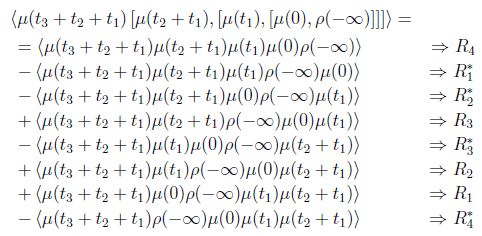
\includegraphics[width = 0.7 \textwidth]{\currfiledir/Feynman1.JPG}
    \caption{Terme der Nichtlinearen Antwort dritter Ordnung}
    \label{fig:Feynman1}
\end{figure}
\begin{figure} [h]
    \centering
    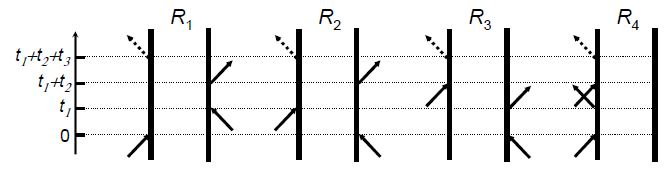
\includegraphics[width = 0.9 \textwidth]{\currfiledir/Feynman2.JPG}
    \caption{resultierendes Feynman-Diagramm}
    \label{fig:Feynman2}
\end{figure}

\paragraph{Beispiel 2:} drei zeitlich versetzte Laserpulse (siehe Abb. \ref{fig:Feynman3})

\begin{figure} [h!]
    \centering
    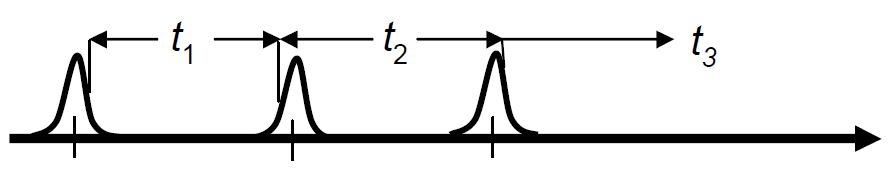
\includegraphics[width = 0.9 \textwidth]{\currfiledir/Feynman3.JPG}
    \caption{Pulsabfolge}
    \label{fig:Feynman3}
\end{figure}

Das sich ergebende E-Feld ist die Summe aus den drei einzelnen Pulsen.
\begin{equation}
    E(t) = E_1(t)\cdot(e^{-i\omega t} + e^{+i\omega t}) + E_2(t)\cdot(e^{-i\omega t} + e^{+i\omega t}) + E_3(t)\cdot(e^{-i\omega t} + e^{+i\omega t})
\end{equation}
Daraus würde folgen, dass insgesamt 6$\cdot$6$\cdot$6$\cdot$4=864 Terme berücksichtigt werden müssten.\\
Diese Zahl kann durch Tricks vermindert werden:
\begin{enumerate}
    \item \textbf{Time ordering:} Die Reihenfolge der Pulse wird berücksichtigt. Das schränkt die Anzahl der Terme auf 32 ein.
    \item \textbf{Rotating Wave Approximation:} Entweder $e^{-i\omega t}$- oder $e^{+i\omega t}$-Terme tragen bei, aber nie beide gleichzeitig. Die Anzahl der Terme beträgt noch 4.
    \item \textbf{Phase Matching:} Jetzt werden zusätzlich noch die Wellenvektoren mitgenommen. Das E-Feld wird zu
    \begin{align}
    E(t) &= E_1(t)\cdot(e^{-i\omega t+ikr} + e^{+i\omega t-ikr}) + E_2(t)\cdot(e^{-i\omega t+ikr} + e^{+i\omega t-ikr}) \notag\\ &+ E_3(t)\cdot(e^{-i\omega t+ikr} + e^{+i\omega t-ikr})
     \end{align}
     Daraus folgt, dass es zwei verschiedene Möglichkeiten zur Aufsummierung der k-Vektoren gibt $k = k_1 \pm k_2 \pm k_3$, wobei nur eine Option am Ende überlebt.
     \begin{figure} [h]
    \centering
    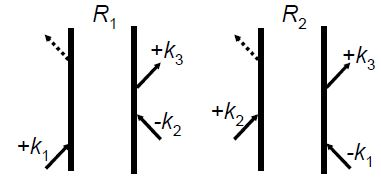
\includegraphics[width = 0.9 \textwidth]{\currfiledir/Feynman4.JPG}
    \caption{Die beiden Möglichkeiten, die Wellenvektoren aufzusummieren.}
    \label{fig:Feynman4}
\end{figure}
\end{enumerate}
Am Ende sind nur noch \textbf{zwei} Komponenten zu beachten.


\section{10.5. Pump-Probe Spectroscopy\protect\footnote{Hamm 2005,  Kap. 4.1}\hfill **} 

Wie beschreibt man mit dem eben eingeführten Formalismus
Zwei-Puls-Experimente?


\section{10.6. {2D}-Spektroskopie\protect\footnote{Hamm 2005, Kap. 7}\hfill ***} 

Wie beschreibt man 3-Puls-Experimente? Wie findet man so
Kopplung zwischen Zuständen, nicht nur Eigenenergien?
 



%-------


\part{Nano Optics and Plasmonics}

\chapter{Overview Nano Optics}




Surface plasmons

Photonic crystals / dispersion relation

Drexhage, dipole in front of a mirror: daten vom paper

Nonlinear oscillator model, daten vom paper

TWTL: linear polarisation dependence: image analysis

Plasmon hybridisation / particle on mirror, FP probe



Plasmonic hot spots

LDOS

SHG particle symmetry



%-------

%\nocite{*}

\printbibliography



\end{document}
